\documentclass[aps,prd,twocolumn,10pt,superscriptaddress,nofootinbib,longbibliography,floatfix]{revtex4-2}

\usepackage{amsmath,amssymb,amsfonts}
\usepackage{bm}
\usepackage{graphicx}
\usepackage{xcolor}
\usepackage{hyperref}
\graphicspath{{figures/}}
\hypersetup{colorlinks=true,linkcolor=blue,citecolor=blue,urlcolor=blue}

\newcommand{\dd}{\mathrm{d}}
\newcommand{\Ham}{\mathcal{H}}
\newcommand{\Mom}{\mathcal{M}}
\newcommand{\MAH}{M_{\rm AH}}

\begin{document}

\title{Black-hole growth in an expanding collisionless medium:\\ Scope, an exact benchmark, baselines, and the verified capability (working note v3)}

\author{Track D of the numerical-relativity particle-in-cell cosmology program}

\date{Working note v3, state of 25 November 2026, the package of the capability gate}

\begin{abstract}
A black hole born in a matter-dominated universe grows by swallowing the collisionless dark matter that falls back onto it, and the matter that survives the fall forms a dense dress whose shape near the horizon has so far been computed only in Newtonian gravity or around a fixed black hole. The same setting tests a recent claim that black holes gain mass as the universe expands, independently of what they accrete. This working note scopes a program that answers these questions with a particle-in-cell method coupled to numerical relativity, and records its state after the baseline gate. It states the questions and their observables, constructs an exact benchmark in which a black hole sits in a vacuum bubble inside an expanding ball of dust and keeps its mass exactly, and reports the baselines. The benchmark data satisfy the constraint equations at the order of the differences that check them. The relativistic density spike of matter on fixed orbits is reproduced around a nonrotating and a spinning black hole and stays in equilibrium when the code moves its particles; a second, independent sample shows no significant deficit of the counts near the black hole. The Newtonian infall around a seed, computed with particles in the code to sixteen times the initial scale factor, follows shells that feel the same force to better than one per cent and approaches the self-similar solution; the asymptotic power law of the dress lies far inside the radii any such run resolves and remains untested. In full relativity the bubble wall and the matter that falls into the black hole follow the exact solution. The late drift of the horizon mass of a vacuum control came from its outer boundary: moved twice as far out, the control holds its mass to a few parts in a hundred thousand, which is the floor of the null test. A slicing condition designed for expanding matter makes the horizon mass grow even in vacuum and is kept out of the null test. In the first run with dust that reaches the black hole, the horizon mass follows the exact mass of the spherical dust solution to a few tenths of a per cent, and its growth closes against the energy of the particles removed at the horizon to a few parts in a thousand once the vacuum control is subtracted. Long runs to five hundred black-hole masses with distant boundaries then hold the null test at the floor of the horizon finder at two cell sizes, and the growth against the flux holds at three particle numbers and two cell sizes, converging in particle number with the noise of the deposit.
\end{abstract}

\maketitle

\section{Introduction}\label{sec:intro}

A black hole that forms or sits in a universe dominated by pressureless matter is surrounded by matter that is still expanding with the Hubble flow. Shell by shell this matter decelerates, turns around and falls back. Matter with little angular momentum falls into the black hole and makes it grow; matter with enough angular momentum misses the horizon, passes the center and settles into a bound, dense dress. In Newtonian gravity the secondary infall onto a seed is self-similar, and the dress approaches a density profile proportional to $r^{-9/4}$ \cite{Adamek:2019wimp,Boudaud:2021spikes}. Such dresses enter the estimated merger rate of primordial black-hole binaries \cite{Kavanagh:2018dress}. Near the horizon the Newtonian picture fails: around a fixed Schwarzschild black hole the density of a slowly grown spike vanishes at four gravitational radii and peaks above the Newtonian value \cite{Sadeghian:2013spike}, and around a Kerr black hole the spike depends on the spin \cite{Ferrer:2017kerr}. The growth of the black hole itself, and the shape of the dress while the black hole grows, need the full Einstein equations. Full-relativity calculations of black-hole growth in the early universe exist for fluids and scalar fields \cite{deJong:2021pbh,Ning:2026rd}; the literature read so far contains none with collisionless particles.

The same configuration speaks to a separate question. Farrah et al.\ reported that the masses of supermassive black holes grow with the scale factor $a$ as $a^k$ with $k$ near three and attributed this to a cosmological coupling of black holes with vacuum-energy interiors \cite{Farrah:2023coupling}; nonsingular black holes give $k=1$ \cite{Cadoni:2023nonsingular}. The same authors assign $k=0$ to a Kerr black hole, so a vacuum black hole is predicted to keep its mass by both sides of the debate. A black hole in an expanding particle medium, evolved without symmetry assumptions, turns this prediction into a numerical null test with an exact reference.

The numerical-relativity particle-in-cell method of Wu and Most \cite{Wu:2026nrpic} evolves macroparticles on geodesics of a spacetime that their deposited stress-energy sources through the Z4c equations, with moving punctures and an apparent-horizon finder on an adaptive mesh. This program uses a version of that method in the code AthenaK. The work is carried out by large-language-model agents under human direction.

This note records the scoping stage, the baselines that need no new code, which the program's baseline gate has accepted with reservations, and the first evolutions toward the next gate; Fig.~\ref{fig:architecture} shows which parts of the calculation exist, which the code has gained since the scoping, and which are new. Section~\ref{sec:problem} states the three questions and their observables. Section~\ref{sec:setup} constructs the benchmark and describes the method. Section~\ref{sec:tests} reports seven results:
\begin{enumerate}
\item the benchmark data satisfy the constraints at fourth order offline and faster inside the code, and the bubble wall follows its exact motion;
\item the horizon mass of an isolated black hole holds to a measured floor until boundary waves arrive, and a vacuum control with distant boundaries sets the floor of the null test;
\item in the first evolution of the benchmark the wall and the infalling matter follow the exact solution, while the horizon mass departs from its predicted level and drifts late in the run together with its vacuum control, and the standard slicing leaves the dust;
\item a slicing condition designed for expanding matter makes the horizon mass of a vacuum black hole grow, and is kept out of the null test;
\item in the first run with dust that reaches the black hole, the horizon mass follows the exact mass of the dust solution and its growth closes against the energy removed at the horizon;
\item the probe-limit spike is reproduced around nonrotating and spinning black holes and stays in equilibrium on the code's geodesics;
\item at the scales a full-relativity run reaches, the black hole captures nearly all infalling matter, and particles in the code's Newtonian mode follow the shell calculation of the infall to sixteen times the initial scale factor and approach the self-similar solution.
\end{enumerate}
Section~\ref{sec:plan} gives the plan and what is open. Table~\ref{tab:parameters} holds the parameters, and Tables~\ref{tab:ledger1}--\ref{tab:ledger10} every number of the note with the registered run that produced it.

\begin{figure*}
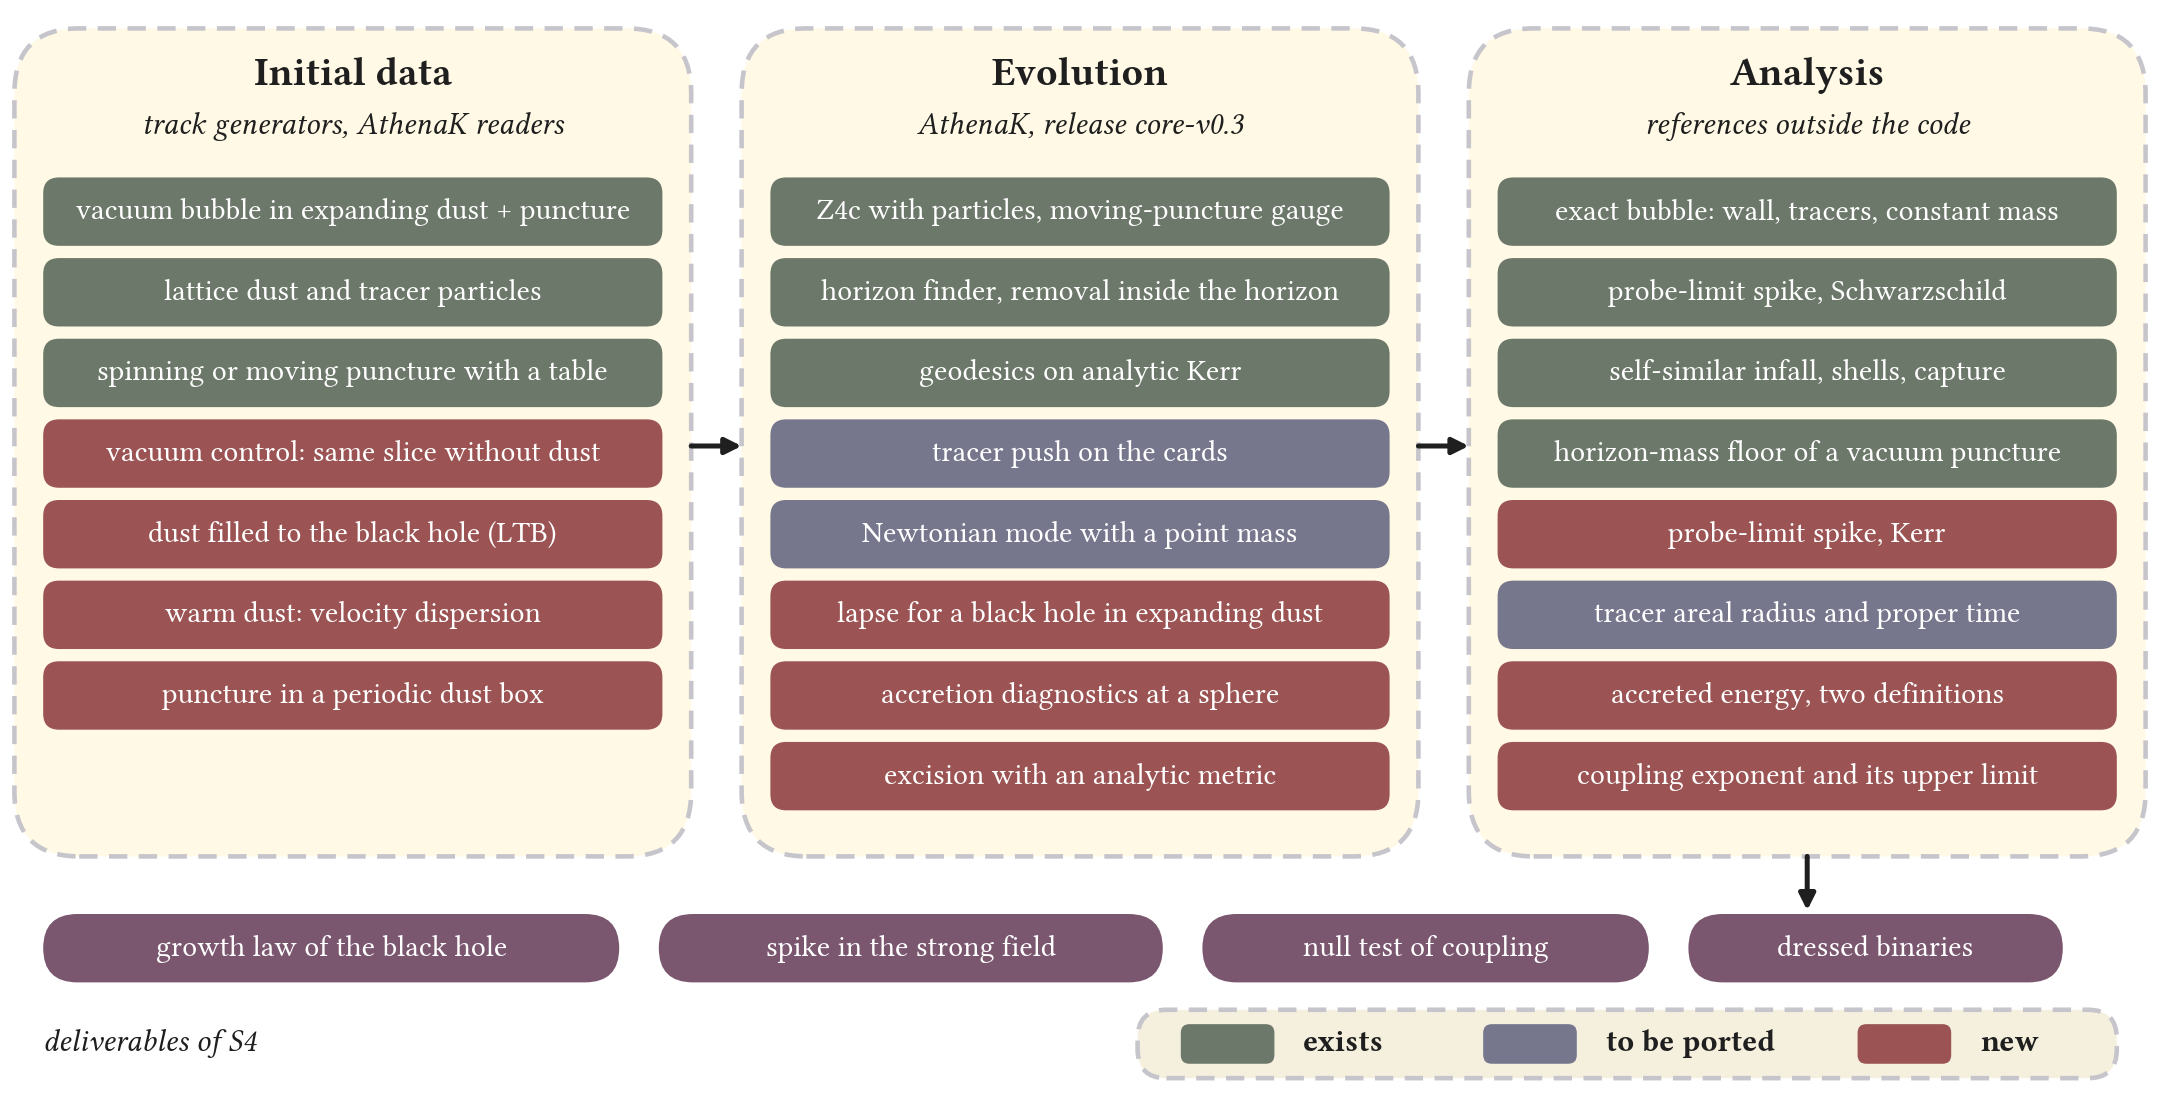
\includegraphics[width=\textwidth]{schem_architecture.png}
\caption{Architecture of the calculation. Each column lists the parts of one stage: initial data, evolution in AthenaK, and analysis against references. Green parts exist, slate parts are tested additions to the code made for this track, red parts are new. The row below gives the chain of runs toward the growth law and the null test with the state of each (green: done; olive: run, with a finding that changed the plan); the violet pills are the deliverables.}
\label{fig:architecture}
\end{figure*}

\section{Three questions}\label{sec:problem}

\subsection{Growth law}

The first question is how fast the black hole grows. The observable is the apparent-horizon mass,
\begin{equation}
\MAH=\sqrt{A/16\pi},
\end{equation}
with $A$ the area of the apparent horizon, against the scale factor measured by distant dust: the areal radius of a comoving dust shell against the proper time of its particles. Coordinate time is gauge dependent and is used only for bookkeeping. In Newtonian gravity the mass that has turned around grows, once the seed is small against it, as
\begin{equation}
M_{\rm ta}-M\simeq\left(\frac{4}{3\pi}\right)^{2/3}M\,\frac{a}{a_i},
\end{equation}
with $M$ the seed mass and $a_i$ the scale factor at the start; the approach to this rate is slow (Sec.~\ref{sec:tests}). Cold matter that falls radially from turnaround is captured, so a cold run measures the growth law directly. The first check of a run is internal: the growth of the horizon mass must equal the energy carried in by the particles that cross the horizon.

\subsection{Spike in the strong field}

The second question is the density of the bound matter within some tens of gravitational radii. A particle that falls from rest at large distance is captured when its specific angular momentum satisfies
\begin{equation}
L<4M,
\end{equation}
the capture condition of a Schwarzschild black hole of mass $M$. Matter that turns around at a radius $r_{\rm ta}$ survives the fall only with a tangential speed above about $4M/r_{\rm ta}$. A run in full relativity reaches turnaround radii of tens of $M$ (Table~\ref{tab:ledger5}), where this speed is a sizable fraction of the speed of light. The spike is therefore a question about warm or rotating matter, and the Newtonian $r^{-9/4}$ dress and the strong-field spike belong to different regimes.

\subsection{Null test of cosmological coupling}

The third question is whether the horizon mass of a vacuum black hole changes with the expansion beyond what it accretes. Writing $M\propto a^k$, a run gives the estimator
\begin{equation}
k_{\rm eff}=\frac{\Delta\ln\left(\MAH-\Delta M_{\rm in}\right)}{\Delta\ln a},
\end{equation}
with $\Delta M_{\rm in}$ the energy that crossed the horizon, measured in two ways: from the particles removed at the horizon, and from the change of the Misner-Sharp mass on a surrounding sphere minus the flux through it. The difference of the two is a systematic error. A floor far above the measured one still bounds $|k|$ far below one over a doubling of $a$, so the test is limited by systematics. In a neighborhood filled with matter the area mass itself drifts: for a McVittie black hole in an Einstein-de Sitter background \cite{Gaur:2023flrw}
\begin{equation}
\frac{\dd\ln\MAH}{\dd\ln a}=-12\,(MH)^2,
\end{equation}
with $H$ the Hubble rate. Inside a vacuum bubble this term is absent.

An upper limit on $k_{\rm eff}$ shows that the method creates no spurious coupling, and that a vacuum black hole in an expanding particle medium behaves as Birkhoff's theorem and the exact solutions require. Its scope is the vacuum black hole: black holes with matter or vacuum energy inside the horizon, the averaging argument that links coupling to dark energy, and the observed black holes lie outside it.

\section{Set-up}\label{sec:setup}

\subsection{Black hole in a vacuum bubble}

The benchmark cuts a vacuum bubble out of a marginally bound, expanding ball of dust and places a black hole at its center, in the manner of Einstein and Straus; outside the ball the spacetime is Schwarzschild of the total mass. The innermost dust shell, the wall, is comoving, so the mass inside it stays constant, and by Birkhoff's theorem so does the mass of the black hole. A marginally bound shell starting at areal radius $R_{\rm in}$ moves on the wall law
\begin{equation}
R_w(\tau)=\left[R_{\rm in}^{3/2}+\tfrac{3}{2}\,(2M)^{1/2}\,\tau\right]^{2/3},
\end{equation}
with $\tau$ the proper time of its particles. Every number of the benchmark thus has an exact value: the horizon mass is $M$ on every spherical slice, and every shell follows its own Lema\^itre-Tolman-Bondi motion.

The initial slice is conformally flat, $\gamma_{ij}=\psi^4\delta_{ij}$, with
\begin{equation}
\psi=1+u+\frac{m_p}{2\bar r},
\end{equation}
where $\bar r$ is the conformal radius, $u$ a regular function, $m_p$ the bare mass of the puncture, and $R=\psi^2\bar r$ the areal radius. Near the black hole the slice is the time-symmetric Schwarzschild slice; across the bubble the extrinsic curvature rises as $K^\theta{}_\theta=-f\,(2M/R^3)^{1/2}$, with a smooth slicing function $f$ that goes from zero to one, and in the dust the slice is the comoving Einstein-de Sitter slice with $K^r{}_r=K^\theta{}_\theta=-H$. Smooth dust edges keep the data infinitely differentiable. Figure~\ref{fig:es} shows the slice and the exact motion of its shells; Table~\ref{tab:parameters} lists the parameters. The wall lies some tens of $M$ out, so that the expansion time is long against the time on which the black hole settles, and the dust stays far from the finely resolved region around the puncture.

\begin{figure*}
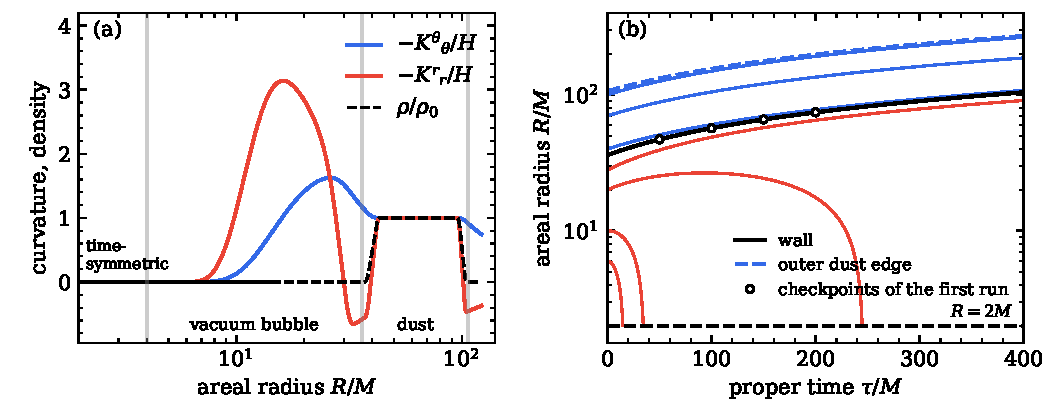
\includegraphics[width=\textwidth]{fig_es.pdf}
\caption{Black hole in a vacuum bubble inside expanding dust. (a) Extrinsic curvature in units of the plateau Hubble rate $H$ and dust density from the Hamiltonian constraint, against areal radius; grey lines mark the regions of Table~\ref{tab:parameters}. (b) Exact areal radius against proper time: wall (black), outer dust edge (dashed), dust shells (blue), tracers that fall into the black hole (red); circles mark the checkpoints of the first run.}
\label{fig:es}
\end{figure*}

\subsection{Black hole in dust that reaches it}

The growth law needs dust down to the black hole. The same construction with the bubble shrunk to a few $M$ gives a slice in which every shell carries the energy of the unperturbed Hubble flow around a point mass. This holds exactly when the black hole carries the mass of the removed dust core in addition to $M$; each shell then follows the radial Kepler law in proper time and areal radius, and the horizon mass on any spherical slice is the mass of the shell that sits at $R=2m$. The Newtonian shells of Sec.~\ref{sec:tests} are the reference for this set-up at large radii, and the exact dust solution near the black hole. A data set of this kind, with the bubble shrunk to a few $M$ and dust down to it, has been built, checked by a second agent, and run once (Sec.~\ref{sec:tests}).

\subsection{Numerical methods}

The spacetime is evolved with the Z4c equations in AthenaK, with $1+\log$ slicing and a Gamma-driver shift around a moving puncture, on a mesh refined around the black hole. Particles move on geodesics of the evolved metric, interpolated to their positions, and their stress-energy is deposited on the mesh. The initial data enter as radial tables of $u$, $K^r{}_r$ and $K^\theta{}_\theta$ superposed with a puncture; dust particles sit on a cubic lattice and carry the exact density. Tracers that follow the motion without sourcing it carry a negligible rest mass, so that they move on timelike geodesics. The apparent-horizon finder uses derivatives of the interpolated metric, and particles inside a fixed fraction of the found horizon are removed. The code now also records every removed particle and counts the particles and the energy that cross spheres around the black hole; these give the two definitions of the accreted energy. Two defaults of the code differ from these settings and are set explicitly in every input. If the $1+\log$ slices followed the dust, the lapse along it would grow as
\begin{equation}
\alpha=1+6\ln a,
\end{equation}
so that a step of coordinate time, which the finest cell fixes, would advance the dust by $\alpha$ times as much proper time, and the lapse could send a front from a dust edge toward the black hole. The first run shows that the slices leave the dust instead (Sec.~\ref{sec:tests}). A slicing condition that lets the lapse relax toward one wherever it exceeds one, on a time short against the expansion time, was added to the code to keep the slices with the dust. Its runs show what it does around a black hole: on a slice whose normal observers diverge, as they do in the vacuum around the black hole, the relaxation holds the lapse of the whole vacuum region above its reference, the coordinates stretch, the horizon shrinks in coordinate size, and with too few cells across it its mass drifts (Sec.~\ref{sec:tests}). Switching the relaxation off around the tracked black hole reduces this drift only in part. The null test and the long runs therefore use the plain $1+\log$ condition, and a cure of the relaxed lapse is an open item of the code.

\section{Tests so far}\label{sec:tests}

\subsection{The benchmark and its constraints}

The construction was checked symbolically, identity by identity, twice. The data satisfy the Hamiltonian and momentum constraints at the order of the differences that check them (Fig.~\ref{fig:constraints}): in a radial check every region away from the puncture converges at fourth order, and in a three-dimensional check in seven cubic boxes the largest residuals converge at fourth order as well. Inside AthenaK, at the start of an evolution, the code's own residuals fall faster than fourth order in the middle of the curvature transition, where its derivative stencils are of higher order; at the inner dust edge the momentum residual converges more slowly, near third order, and near the puncture the Hamiltonian residual is of order one at both spacings, as expected at a puncture. The density deposited by the lattice particles equals the exact density to rounding error. Evaluated directly on the table columns, the Hamiltonian constraint returns the plateau density to rounding error and zero density in the exterior; inside the bubble it returns a small density that grows fourfold when the table spacing doubles, the truncation error of the second-order differences used for this check. The wall column of the reference agrees with the wall law to rounding error, and the mass inside the wall is exactly $M$. The tracers released in the transition start with the expansion of the slice; their arrival at $R=2M$ follows the infall law of their own energy, which is what the first run compares with.

\begin{figure*}
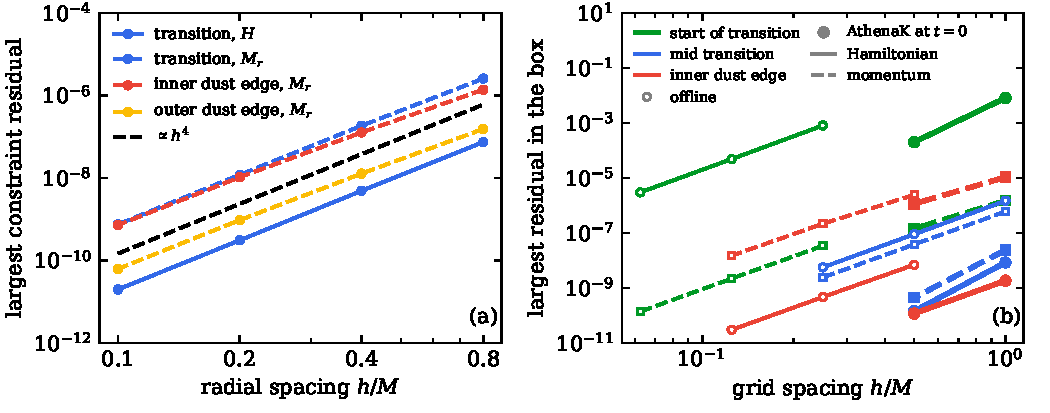
\includegraphics[width=\textwidth]{fig_constraints.pdf}
\caption{Constraint residuals of the benchmark data against the grid spacing. (a) Radial check with fourth-order differences in the regions of the slice; the dashed line is proportional to $h^4$. (b) Cubic boxes in three dimensions: offline check (open markers, thin lines) and the residuals AthenaK computes at the start (filled markers, thick lines); solid lines Hamiltonian, dashed lines momentum constraint.}
\label{fig:constraints}
\end{figure*}

\subsection{Horizon-mass floor}

The null test needs to know how well the code holds the mass of a black hole whose mass is constant. An isolated puncture of unit mass, the black hole of the benchmark without the dust, was evolved to $500M$ at two resolutions (Fig.~\ref{fig:floor}). After the initial gauge transient the horizon mass sits slightly above $M$ at the coarser resolution and slightly below at the finer one. At the finer resolution the running mean holds to the floor of Table~\ref{tab:ledger2} until about $210M$; between $220M$ and $255M$ both resolutions show the same excursion, of the same size, which marks it as a disturbance from outside the black hole; its attribution to the outer boundary remains to be tested. The smallest detectable change, the sum of the largest drift of the running mean, the spread between finder settings and twice the scatter, is the floor of the null test for windows that end before the excursion. The measured spin stays many orders of magnitude below $M^2$. The floor belongs to an asymptotically flat black hole; the benchmark with dust and a different exterior needs its own control with the same mesh and gauge. That control exists: the vacuum control of the first run of the bubble (next subsection), run again with its outer boundary twice as far out, holds its horizon mass from $100M$ to the end of the run to a few parts in a hundred thousand (Table~\ref{tab:ledger8}), a value the independent reviewer of the baseline gate recomputed from the raw finder output. This matched control sets the floor of the null test in place of the isolated black hole: the isolated black hole at the same cell size makes half of its drift from $50M$ on in the end of its gauge transient, and its later excursions remain unattributed.

\begin{figure*}
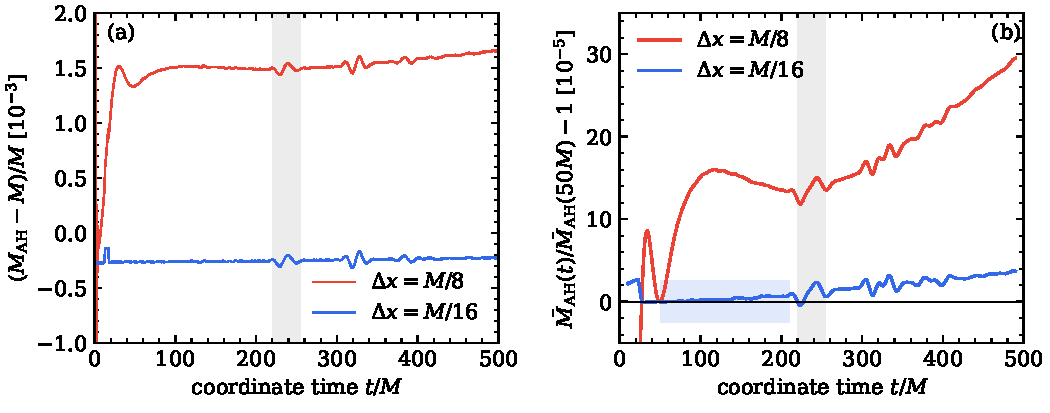
\includegraphics[width=\textwidth]{fig_floor.pdf}
\caption{Apparent-horizon mass of an isolated black hole at two resolutions. (a) Horizon mass minus the bare mass. (b) Running mean over $20M$ relative to its value at $50M$; the blue band is the smallest detectable change at the finer resolution for windows that start at $50M$ and end before $210M$. Grey: the excursion seen at both resolutions.}
\label{fig:floor}
\end{figure*}

\subsection{First evolution of the bubble}

The benchmark was evolved for $200M$ of coordinate time with a finest cell of $M/8$ at the black hole, the outer dust edge moved inward to reduce the cost, together with its vacuum control: the same table without dust, on the same mesh, with the same slicing and length (Table~\ref{tab:parameters}). The predictions were written down before either run; Fig.~\ref{fig:esrun} sets them against the outcome, and Table~\ref{tab:ledger3} gives both.

What held concerns the matter. The wall tracers follow the wall law in their own proper time to a few parts in a thousand over the predicted range, in both runs (Fig.~\ref{fig:esrun}c). Beyond that range the tracers on the coordinate axes and on the diagonals part; since the exact solution is spherical, this anisotropy belongs to the Cartesian mesh or the outer boundary. The tracers released inside the bubble reach $R=2M$ at the proper times of the infall law of their own energy, to a small fraction of $M$, the same in both runs, and are removed at the horizon (Fig.~\ref{fig:esrun}d); the outermost inner group turns around at its exact radius and, in the benchmark run, falls in before the run ends. Every dust particle stays outside the wall along its own direction at every stored time. The two horizon masses agree far below the floor until a signal from the dust can reach the black hole.

What failed concerns the horizon mass and the slicing, and we state it as plainly. First, the level: we predicted that the horizon mass, after the initial gauge transient, would sit above $M$ by the offset the isolated black hole shows at the same cell size; both runs sit lower, at nearly the same level, after a step that both show early in the evolution (Fig.~\ref{fig:esrun}a). The prediction is refuted. The mesh around the black hole is wider than that of the isolated black hole; whether this sets the level is untested. Second, the drift: we predicted that the horizon mass would hold, from $100M$ on, to the floor of the isolated black hole; both runs exceed that floor several times, so this prediction is refuted too. Up to about $165M$ both stay close to it, the benchmark with larger oscillations than the control; after about $165M$ both drift down together, the benchmark more than the control (Fig.~\ref{fig:esrun}b). The criterion fixed in advance would call the dust coupled to the black hole if the benchmark's drift exceeded the control's by more than three times the control's floor; the measured excess stays below twice that floor, so any coupling through the slicing, the deposit or the boundary lies below what this run resolves. For the control the cause of the late drift is now known. The same control with its outer boundary twice as far out follows the first one to rounding error until a signal from the nearer boundary can reach the black hole, separates from it then, and holds its horizon mass to the floor of Table~\ref{tab:ledger8} where the first control falls: the late drift of the control came from its outer boundary, although the lapse at the probes showed no coherent signal moving inward. Whether the larger late drift of the benchmark has the same cause remains to be tested; long runs of the benchmark and of its control with the boundary four times as far out test it (Sec.~\ref{sec:plan}). Third, the slicing: we predicted that the $1+\log$ lapse in the dust would grow as $1+6\ln a$, the homogeneous model; the lapse follows this curve only for the first few $M$, peaks far below it, and late in the run settles near a constant value of order one at every probe outside the black hole (Fig.~\ref{fig:esrun}e). The model is refuted. The trace of the extrinsic curvature at a dust tracer shows why: within some tens of $M$ the slices stop following the dust, and for a while they contract where the dust expands (Fig.~\ref{fig:esrun}f). The dust therefore advances in proper time only somewhat faster than coordinate time, far slower than in the homogeneous model, and a lapse pulse from the dust reaches the black hole and moves its horizon mass for some tens of $M$ before it settles.

\begin{figure*}
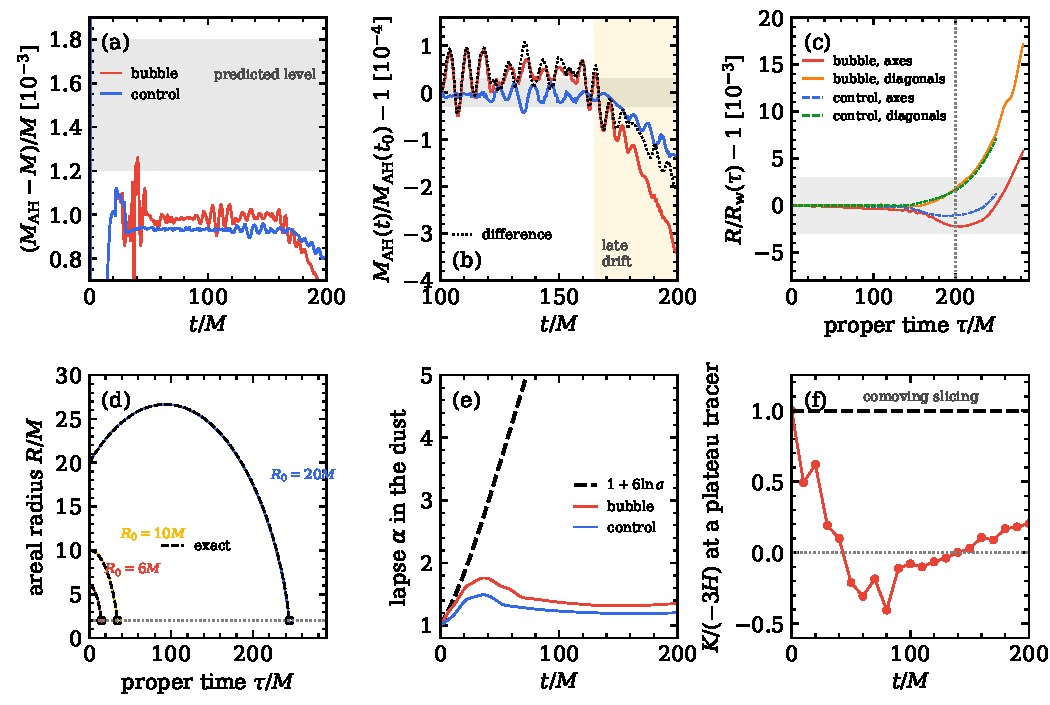
\includegraphics[width=\textwidth]{fig_esrun.pdf}
\caption{First evolution of a black hole in a vacuum bubble (red) and of its vacuum control (blue). (a) Apparent-horizon mass minus $M$; grey band: predicted level. (b) Horizon mass relative to its value at $100M$, and the difference of the two runs (dotted); grey band: predicted bound; shaded: the late drift. (c) Areal radius of the wall tracers over the wall law on the axes and the diagonals; grey band: predicted bound. (d) Infalling tracers against proper time, exact curves dashed, exact arrival at $R=2M$ circled. (e) Lapse in the dust against the homogeneous $1+\log$ model (dashed). (f) Trace of the extrinsic curvature at a dust tracer over its comoving value.}
\label{fig:esrun}
\end{figure*}

\subsection{A slicing for expanding matter, and why the null test does without it}

The relaxed lapse of Sec.~\ref{sec:setup} was run on the vacuum control with distant boundaries and on the benchmark. In vacuum the horizon mass grows over the second hundred $M$ by about a part in a thousand, more than twenty times the floor of the same control with the $1+\log$ condition, and the horizon ends at less than half of its coordinate radius under $1+\log$ (Table~\ref{tab:ledger8}). With dust the growth is larger still, and identical, to a few parts in a billion, whether the boundary lies at the nearer or the farther distance: here the growth comes from the slicing rather than the boundary. The difference between benchmark and control reaches a few parts in a thousand, far above any floor. A null test with this slicing would measure the slicing; the null test and the long runs use $1+\log$.

\subsection{Matter that reaches the black hole}

The data set of Sec.~\ref{sec:setup} with dust down to a few $M$ was evolved for $200M$ with the mesh, slicing and outer boundary of the first run, and compared with the same vacuum control. The predictions and the criteria were written before the run. All held but two: a single finder sample within the first $M$, the initial dip of the finder, lay outside the predicted band, and a criterion on the timing of the removals that we expected to fail held. Figure~\ref{fig:esf} shows the result. The horizon mass grows by a quarter of $M$ in $200M$ (Fig.~\ref{fig:esf}a). Every particle that the code removes inside the horizon carries the energy fixed by the initial data for its shell, and the sum of these energies follows the growth of the horizon mass; the difference between the two settles within the first $20M$ and then stays at about a hundredth of $M$, most of which the finder shows in the vacuum control as well: subtracting the control's history leaves a few parts in a thousand of $M$, about a hundredth of the growth (Fig.~\ref{fig:esf}b; Table~\ref{tab:ledger9}). The exact dust solution gives a second, gauge-invariant reading. Each removed particle belongs to a shell whose Misner-Sharp mass is known, and when the particle is removed the horizon must hold at least that mass: it does, for every one of the removed particles, and the horizon mass at removal equals the exact mass of the shell then at the horizon to a few tenths of a per cent over the whole run (Fig.~\ref{fig:esf}c). Every removal happens between the exact proper time at which its shell crosses $R=2m$ and the time at which it would reach the center. This is the matter criterion of the next gate, that the growth agrees with the integrated flux, met once: at one resolution, for $200M$, with the outer boundary close enough to reach the black hole in the second half of the run. The long run of the same data with distant boundaries repeats it.

\begin{figure*}
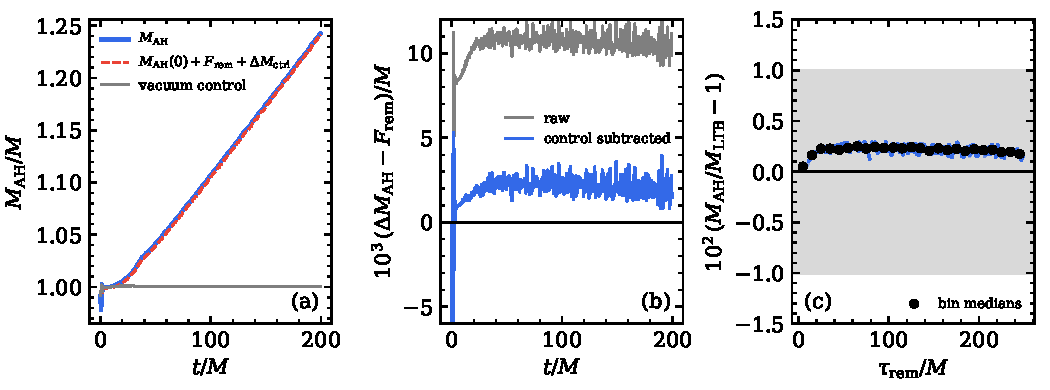
\includegraphics[width=\textwidth]{fig_esf.pdf}
\caption{First run with dust that reaches the black hole. (a) Apparent-horizon mass (blue), its initial value plus the energy of the particles removed at the horizon plus the change of the vacuum control's horizon mass (red, dashed), and the vacuum control (grey). (b) Growth of the horizon mass minus the removed energy, raw (grey) and with the control's history subtracted (blue). (c) Horizon mass at each removal over the exact mass of the dust solution at the proper time of the removed particle, minus one: a tenth of the removals (dots) and the medians in bins of $10M$ (black); grey band: the criterion fixed before the run.}
\label{fig:esf}
\end{figure*}

\subsection{Spike in the probe limit}

Around a fixed Schwarzschild black hole the density of a spike that grows adiabatically follows from matching the actions of the orbits before and after the growth. For a constant distribution function this calculation reproduces the published relativistic profile \cite{Sadeghian:2013spike}: it vanishes at $4Gm$ and peaks above the Newtonian profile of Gondolo and Silk (Fig.~\ref{fig:spike}a). Moving the Newtonian inner edge from $8Gm$ to $4Gm$ overestimates the peak. For a spike grown from a Hernquist cusp, the canonical-action form agrees with the curve of Ferrer et al.\ \cite{Ferrer:2017kerr} (Fig.~\ref{fig:spike}b); the earlier form misses a factor $r^2/\Delta$ that Ferrer et al.\ point out, and lies above it near the peak. A sample of particles drawn from the equilibrium and moved by AthenaK on the analytic Schwarzschild metric for $20\,000M$ keeps the equilibrium counts in every radial shell within their Poisson scatter (Fig.~\ref{fig:spike}c), with energy and angular momentum conserved to high accuracy. Probes placed just inside the capture boundary all cross the horizon and probes just outside all stay out, with crossing times that converge at second order in the time step.

Schwarzschild is the nonrotating limit of the Kerr spike, and the same calculation with the capture boundary and the actions of Kerr orbits \cite{Ferrer:2017kerr} returns the Schwarzschild profile above at zero spin. For a constant distribution function it reproduces the published Kerr spikes at spins $0.5$ and $0.8$, on the equator and on the axis, with the equatorial inner edge at the marginally bound prograde orbit and a peak that rises with the spin (Fig.~\ref{fig:kerr}a). For the spike grown from a Hernquist cusp the agreement holds at zero spin and on the axis; for orbits with angular momentum along the spin our density lies a few per cent below the published curves near the peak (Fig.~\ref{fig:kerr}b). The black-hole mass of these curves is our choice: Ferrer et al.\ quote four million solar masses as a lower bound for the black hole at the Galactic center, and with it our nonrotating curve agrees with theirs. A second agent who implemented the published prescription independently finds nearly the same peak as ours and the same difference from the published curve. The difference grows with the spin, and at the highest spin it sits where the published curve has a narrow bump at its maximum, while the published curves for a constant distribution function, which need no matching of actions, agree with ours. We therefore judge that the difference lies in the published curve or in a detail of its computation that the paper leaves unstated. Moved by AthenaK on the analytic Kerr metric at spin $0.8$ for $20\,000M$, particles drawn from the grown equilibrium keep the counts of every radial range within their Poisson scatter and without trend, and keep the net prograde rotation and the contrast between equator and pole of the equilibrium (Fig.~\ref{fig:kerr}c).

In the three innermost ranges the time-averaged counts of this sample lie a few per cent below the equilibrium, each within one to two standard deviations of a time average over a finite set of orbits. A second sample of the same distribution, drawn with another seed and moved by the same code for the same time, tests whether this is the noise of one sample or a bias of the sampler or of the evolution. We fixed beforehand that a bias would be indicated if the sum of the three inner deviations of the second sample, each in units of its error, fell below $-1.5$. The sum stays above that mark (Fig.~\ref{fig:kerrseeds}; Table~\ref{tab:ledger10}): the second sample lies closer to the equilibrium in all three inner ranges, and the mean of the two samples bounds a bias, at two standard deviations, to several per cent inside $6M$ and to about two per cent between $6M$ and $10M$. In one outer range the second sample lies two standard deviations above the equilibrium, just outside the band we had predicted. One particle of the second sample, the one drawn closest to the edge of the loss cone, crossed the horizon at its first pericenter: the small energy error of the integration carried it across the separatrix. The code version used for both samples, kept the same for the comparison, has no excision on the analytic metric (later versions have it), so the particle then stays at a small radius, and counting it there raises the innermost count by seven tenths of a per cent. Read without it, all three inner ranges lie below the equilibrium in both samples, and their combined deviation stays below two standard deviations. A deficit of one or two per cent inside $10M$ is thus neither shown nor excluded by two samples; a direct test of the sampler with many more particles would decide it.

\begin{figure*}
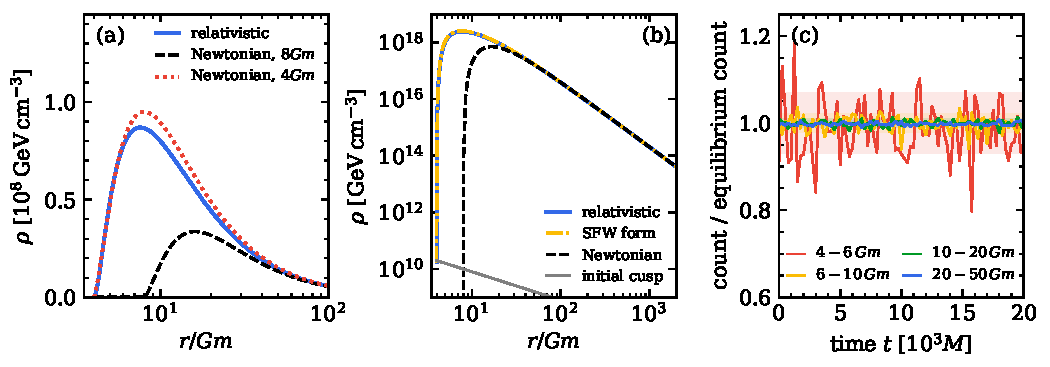
\includegraphics[width=\textwidth]{fig_spike.pdf}
\caption{Density spike of dark matter around a Schwarzschild black hole on fixed orbits. (a) Constant distribution function: relativistic profile and the Newtonian profile cut at $8Gm$ and at $4Gm$. (b) Spike grown from a Hernquist cusp around a black hole of $4\times10^6$ solar masses. (c) Particle counts of the code in four radial shells over the equilibrium count, with bands of one Poisson standard deviation; $M=Gm$.}
\label{fig:spike}
\end{figure*}

\begin{figure*}
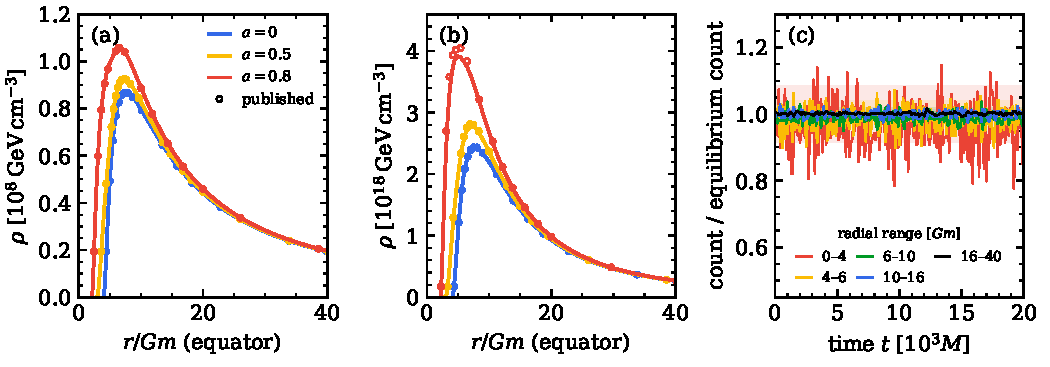
\includegraphics[width=\textwidth]{fig_kerr.pdf}
\caption{Density spike of dark matter around a Kerr black hole on fixed orbits. (a) Constant distribution function on the equator at three spins: our calculation (lines) and the published curves (circles). (b) The same for a spike grown from a Hernquist cusp around a black hole of $4\times10^6$ solar masses. (c) Particle counts of the code at spin $0.8$ in five radial ranges over the equilibrium count, with bands of one Poisson standard deviation; $M=Gm$.}
\label{fig:kerr}
\end{figure*}

\begin{figure*}
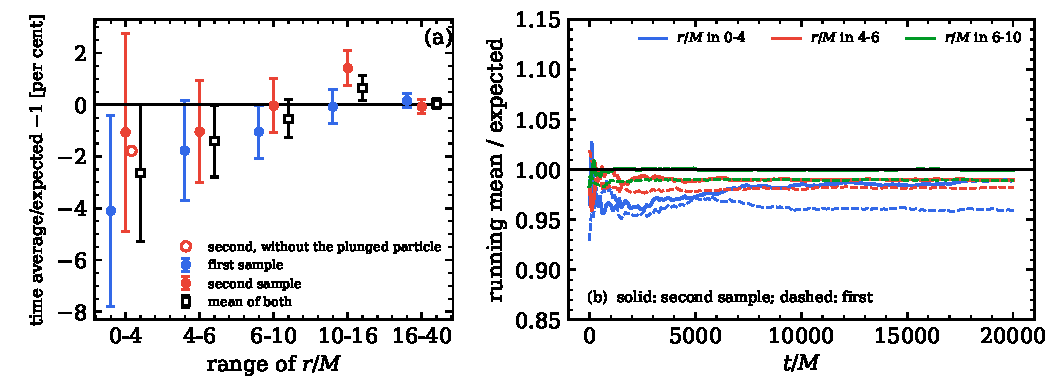
\includegraphics[width=\textwidth]{fig_kerr_seeds.pdf}
\caption{Kerr spike at spin $0.8$ on the analytic metric, two independent samples of $48\,000$ particles each, moved by the code for $20\,000M$. (a) Time-averaged count over the equilibrium count minus one in five radial ranges: first sample (blue), second sample (red; open circle: without the particle that crossed the horizon), and their weighted mean (squares), with the error of a time average over a finite set of orbits. (b) Running time average of the count over the equilibrium count in the three inner ranges, second sample (solid) and first sample (dashed); $M=Gm$.}
\label{fig:kerrseeds}
\end{figure*}

\subsection{Secondary infall and capture}

The Newtonian infall around a seed in an Einstein-de Sitter background sets the scales of the full-relativity runs. The self-similar solution approaches the $r^{-9/4}$ power law only deep inside the turnaround radius (Fig.~\ref{fig:infall}a): the apocenters of a shell shrink over many orbits, so the local slope reaches its asymptotic value only several decades in. At the radii a run resolves, from a few thousandths to a few tenths of the turnaround radius, the profile is steeper. The shell calculations give the turned-around mass, the mass of a black hole that absorbs radial dust, and the mass of the dress that forms when the dust may pass the center (Fig.~\ref{fig:infall}b). They agree with a closed form computed independently. The black hole doubles its mass within a few doublings of the scale factor, and the approach of the turned-around mass to its asymptotic rate takes two decades in $a$. Warm dust shows how small the dress stays at reachable scales (Fig.~\ref{fig:infall}c): with an initial dispersion of a few hundredths of the speed of light all collapsed dust is captured, and even at the largest dispersion considered about three quarters of it is. The cold runs therefore measure the growth law, and a surviving dress requires tangential speeds that also change the infall itself.

\begin{figure*}
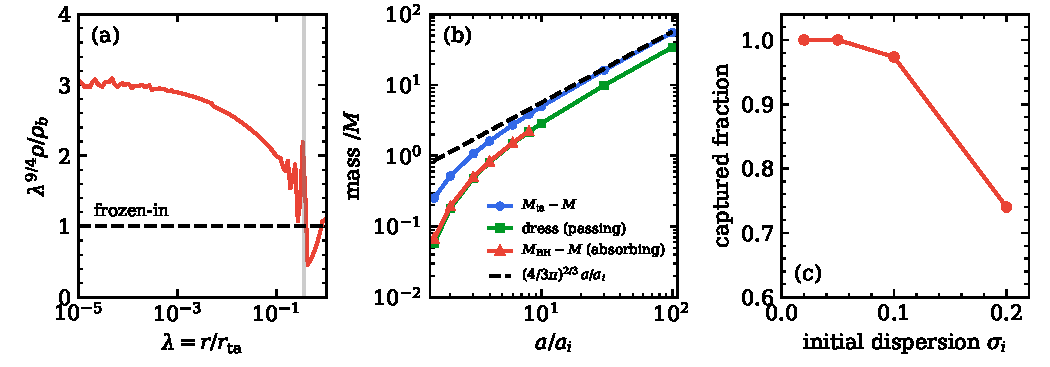
\includegraphics[width=\textwidth]{fig_infall.pdf}
\caption{Newtonian secondary infall onto a seed of mass $M$ in a matter era. (a) Self-similar density over the frozen-in power law $\lambda^{-9/4}$ (dashed) against $\lambda=r/r_{\rm ta}$; the grey line marks the outermost caustic. (b) Turned-around mass, dress of passing dust, and black-hole mass for absorbed radial dust; dashed: the asymptotic rate. (c) Captured fraction at $a/a_i=4$, $\epsilon=0.01$, against the initial dispersion.}
\label{fig:infall}
\end{figure*}

The same infall computed with particles in the Newtonian mode of the code reproduces the shell calculation (Fig.~\ref{fig:newton}). The seed is a compact clump of particles at the center of a cell, where its own field holds it in place; a fixed point mass, now a tested addition to the code, will replace it. At three cell sizes the turned-around mass agrees with shells that feel the measured force law of the mesh to a few parts in a thousand throughout (Fig.~\ref{fig:newton}a,b). The dress agrees with them to about one per cent once it has formed, from about three times the initial scale factor on; while it is young and small it lies a few per cent above them, by an amount that depends on the force law near the center. The density profile agrees with the matched shells within the scatter of its bins from four cells out to the turnaround radius, except at the outermost caustic, where a small part of the dress extends beyond the caustic of the shells, for a reason still open. Against the self-similar solution the profile agrees only in the outer part of the turnaround region and is flatter inside, where the seed still dominates (Fig.~\ref{fig:newton}c); even in the outer part, the deviation at the latest time depends on the turnaround radius used to scale the profile (Table~\ref{tab:ledger6}). The dress holds a smaller share of the turned-around mass than in the self-similar limit and approaches it slowly.

\begin{figure*}
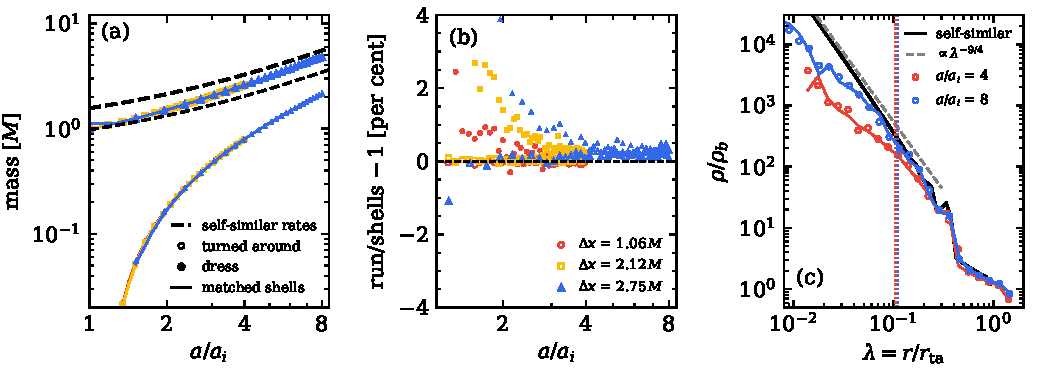
\includegraphics[width=\textwidth]{fig_newton.pdf}
\caption{Secondary infall onto a seed of mass $M$ computed with particles in the Newtonian mode of the code at three cell sizes. (a) Turned-around mass (open) and dress (filled) against the scale factor; lines: shells that feel the force law of the mesh; dashed: the self-similar rates. (b) Run over matched shells minus one. (c) Density over the background against radius in units of the turnaround radius at $a/a_i=4$ and $8$, with matched shells (lines), the self-similar solution and the power law $\lambda^{-9/4}$; dotted lines mark four cells.}
\label{fig:newton}
\end{figure*}

A larger run, with a coarser cell in a larger box, follows the infall to sixteen times the initial scale factor and keeps every particle (Fig.~\ref{fig:q16}). Against shells that feel the cell-centred force of the mesh, its turned-around mass stays within half a per cent and its dress within one per cent from three to twelve times the initial scale factor (Fig.~\ref{fig:q16}b). At sixteen times the turned-around mass lies almost one per cent above the shells, outside the band we fixed before the run; we attribute this, without a test, to the outermost turned-around shells, whose energies the coarse start of the run changed (Table~\ref{tab:ledger7}). The ratio of dress to turned-around mass rises toward its self-similar value, and the turned-around mass per unit scale factor falls toward the asymptotic rate, as for the shells. At sixteen times the initial scale factor the density lies within about a sixth of the self-similar solution in every one of six bins from four cells to a third of the turnaround radius, and within a twelfth in the root mean square (Fig.~\ref{fig:q16}c); as at eight times, that bound depends on the turnaround radius that scales the profile. The independent reviewer of the baseline gate recomputed the turned-around mass with two estimators of its own and found the same value to a tenth of a per cent. The run has one resolution; a second, with finer cells, is running.

\begin{figure*}
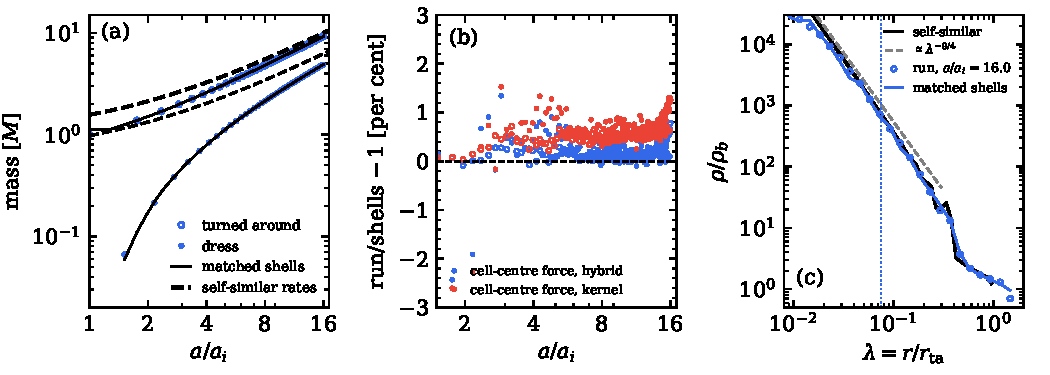
\includegraphics[width=\textwidth]{fig_q16.pdf}
\caption{Secondary infall onto a seed of mass $M$ in the Newtonian mode of the code to sixteen times the initial scale factor. (a) Turned-around mass (open) and dress (filled) against the scale factor; black lines: shells that feel the cell-centred force of the mesh; dashed: the self-similar rates. (b) Run over matched shells minus one, for two models of the cell-centred force; open: turned-around mass, filled: dress. (c) Density over the background against radius in units of the turnaround radius at the last time, with the matched shells, the self-similar solution and the power law $\lambda^{-9/4}$; dotted: four cells.}
\label{fig:q16}
\end{figure*}

What this baseline tests, and where it stops. The track sheet asked the particle run to reproduce the $r^{-9/4}$ profile of the self-similar infall. The self-similar solution with a seed reaches that slope only below about a ten-thousandth of the turnaround radius (Fig.~\ref{fig:infall}a). At sixteen times the initial scale factor the run resolves radii down to a thirteenth of the turnaround radius, nearly three decades above, and its local slope there agrees with the slope of the self-similar solution on the same bins, not with $-9/4$ (Table~\ref{tab:ledger7}); a mesh that resolves the power law would need scale factors far beyond any run. The criterion of this baseline was therefore changed after the first runs, by a ruling of the program, to the growth of the turned-around mass and the dress against matched shells and the approach of the profile to the self-similar solution, judged from three times the initial scale factor on. The power law itself is not tested by any run of this note, and the agreement above is not a confirmation of it.

\section{Verified capability}\label{sec:g2}

The second gate asks for the capability before the science: the null test and the growth criterion of the track, run long enough and with distant enough boundaries to be read without the boundary signal, and three-way convergence in particle number, cell size and boundary or gauge. Every run of this section slices with the $1+\log$ condition and the Gamma-driver shift, has its outer faces at $\pm768M$, and was made without the finder's status record; each failed search leaves a signature in the finder's output (a repeated line or no value), and no horizon number below rests on one (Table~\ref{tab:ledger11}).

\subsection{Null test to $500M$}

The benchmark and its vacuum control ran to $500M$ at $M/8$ and to $300M$ at $M/16$. With the finder of the production runs, the bubble's horizon mass departs from the control's by at most $2.3\times10^{-4}$ of $M$ after $100M$, below the threshold fixed before the runs (Table~\ref{tab:ledger11}). Searched again with a tighter stopping rule, the difference falls to at most $7.3\times10^{-5}$ at $M/8$ (over $100$--$500M$) and $5.5\times10^{-5}$ at $M/16$ (over $100$--$300M$) and shows no trend in time: the remaining floor belongs to the finder. At $M/4$ the same test fails, the difference growing to several parts in a thousand by $300M$; the horizon there spans eight cells, and that mesh lies outside the regime in which the null test converges. We state the mesh leg of the null test with two members and no order, because both sit at the floor and there is no error above it whose order a third member could measure.

\subsection{Growth against the flux at three particle numbers}

The run with dust that reaches the black hole was repeated with a quarter and with four times the number of particles, keeping horizon excision on to the end. At every particle number the horizon mass at each removal equals the exact mass of the shell then at the horizon to three tenths of a per cent in every bin of proper time to $500M$, and the growth stays within the band of the flux criterion at every sample (Table~\ref{tab:ledger11}). The energy removed at the horizon agrees with that of the middle member to better than one per cent after $100M$. Fig.~\ref{fig:g2conv}a shows the differences of the horizon masses between neighbouring members: the coarser pair differs by more at each of the four times we named beforehand, and over windows of $50M$ its scatter is two to three times that of the finer pair, the factor two that sampling noise falling as $N^{-1/2}$ gives. The constraint residual outside the horizon behaves the same way: on the plane $z=0$ between $1.2$ horizon radii and $30M$ it doubles with a quarter of the particles and halves with four times as many. It is the sampling noise of the deposit.

\subsection{Growth against the flux at two cell sizes}

The same data with a finest level of $M/16$ around the black hole meets the flux criterion to $300M$ with the vacuum control of its own mesh. The growth $\Delta M = \MAH(t)-\MAH(20M)$ of the two meshes inside the regime agrees to a few parts in ten thousand at $100$, $200$ and $300M$ (Fig.~\ref{fig:g2conv}b,c). These samples understate the difference: over $150$--$299M$ the $M/16$ member lies systematically above, by $5.8\times10^{-4}$ on average over $250$--$299M$ and by at most $1.0\times10^{-3}$, well inside the tolerance of the flux criterion, and subtracting each mesh's vacuum control does not remove this offset (Fig.~\ref{fig:g2conv}c). The $M/4$ member is drawn for completeness and departs by one to four parts in a thousand; it carries no weight, and with two members inside the regime no order of convergence is claimed. Both meshes show the same step of the bin medians of a few tenths of a per cent when horizon excision ends at four times its initial radius; the run that keeps excision on has no step.

\begin{figure*}
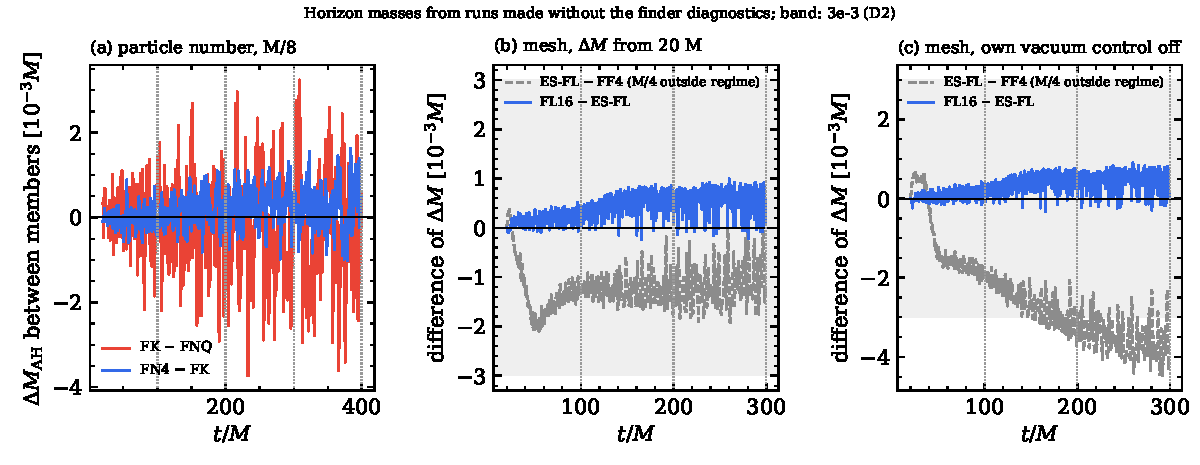
\includegraphics[width=\textwidth]{fig_g2conv.pdf}
\caption{Three-way convergence of the growth. (a) Differences of the apparent-horizon mass between the runs with $N/4$ and $N$ particles (red) and between $4N$ and $N$ (blue), all at $M/8$. (b) Differences of the growth $\Delta M$ from $20M$ between $M/16$ and $M/8$ (blue) and between $M/8$ and $M/4$ (grey, dashed; $M/4$ lies outside the convergent regime). (c) As (b) with each mesh's own vacuum control subtracted. Grey band: the tolerance of the flux criterion, $3\times10^{-3}M$; dotted lines: the times named before the runs. Horizon masses from runs made without the finder's status record.}
\label{fig:g2conv}
\end{figure*}

\subsection{What stays open at this gate}

The gauge leg of the convergence has one member: the relaxed lapse makes the horizon mass of a vacuum black hole grow and cannot serve, so the third axis is the boundary, with faces at three distances. Once the black hole has grown, horizon excision removes some dust up to two thirds of $M$ of proper time before its exact crossing. A second agent traced this to the shells rather than to the excision: the numerical shells run ahead of the exact solution by about $0.2$ per cent of their proper time at an initial radius of $28M$ ($0.78M$ at $M/8$, $0.55M$ with four times the particles, $0.40M$ at $M/16$), so they reach the horizon early; this is shown for the tracers and inferred for the dust from the same timing. The lead converges with both the cell size and the particle number, moves the horizon-mass criterion by less than a tenth of its tolerance, and is a bias of any profile read from removal times. With a quarter of the particles one gauge-invariant check fails late: after about $220M$ a quarter of the removals find the horizon mass slightly below the exact mass of their shell. These failures are on record with the predictions that preceded them.

\section{Plan and open items}\label{sec:plan}

The baselines passed the program's gate with reservations, and three of them shape what follows. The infall baseline rests on one resolution and thin margins, and the power law it was first meant to show remains untested (Sec.~\ref{sec:tests}). The comparison with the published Kerr spike at the highest spin rests partly on our judgement that the difference lies in the published curve. And the null test must quote the floor of its own matched control, not that of the isolated black hole, and must stay off the relaxed lapse.

At the second gate the questions met their first long runs (Sec.~\ref{sec:g2}). The null test holds to $500M$ at two cell sizes with the boundaries four times as far as in the first run, and its floor is set by the stopping rule of the horizon finder; the growth against the energy removed at the horizon holds at three particle numbers and two cell sizes inside the convergent regime, to $400$--$500M$. The relaxed lapse makes the horizon mass of a vacuum black hole grow and is kept out of every run until the code has a cure.

Toward the third gate five items are open, and the scope of that gate is written around them. The mesh leg has two members inside the convergent regime and no order; a third member is needed, with the horizon inside the finest level for the whole run. There is no gauge leg in the slicing, because the one alternative slicing at hand fails near a black hole. Every horizon mass of the second gate was made without the finder's status record and with its production stopping rule; the code now offers a converged rule with that record, and the next runs use it. Horizon excision must stay on while the black hole grows, which the code's new guard on the excision radius is meant to ensure. And the shells run ahead of the exact solution by about $0.2$ per cent of their proper time, a lead that converges but must be measured and carried as a bias in every profile read from removal times. Two reservations of the first gate also remain: the infall baseline has one resolution, and its approach to the self-similar solution between a hundredth and a sixteenth of the turnaround radius remains to be shown; the comparison with the published Kerr spike at the highest spin rests partly on judgement.

The null test will give an upper limit on the coupling exponent of a vacuum black hole in an expanding particle medium. The statement covers ordinary black holes, whose interior is vacuum: black holes with matter or vacuum energy inside the horizon, the averaging argument that links coupling to dark energy, and the observed black holes lie outside it, so the test bears on the method and on the vacuum solutions, and leaves the hypothesis for the objects its authors consider to other evidence. Figure~\ref{fig:timeline} places these items between the gates.

\begin{figure*}
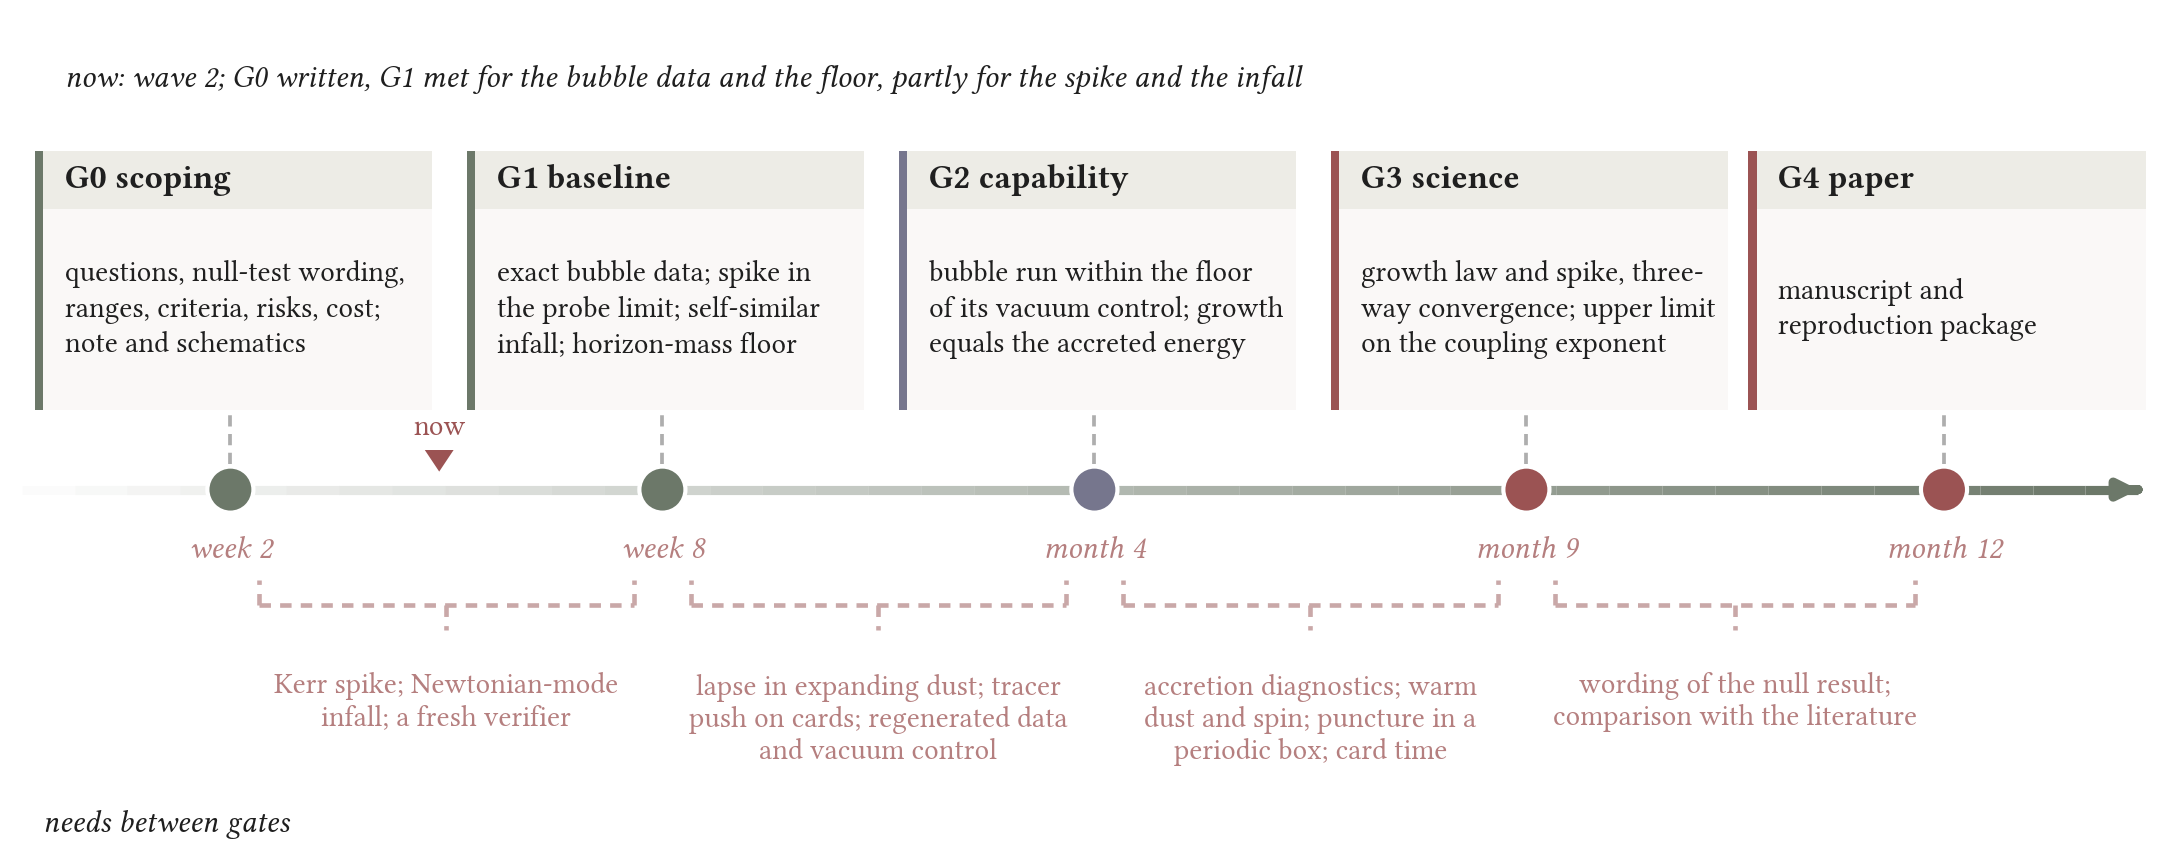
\includegraphics[width=\textwidth]{schem_timeline.png}
\caption{Stages of the track. The five gates with what each requires and the state reached, the present position, and what is needed between gates; the time labels are the program's targets.}
\label{fig:timeline}
\end{figure*}

\section{Summary}\label{sec:summary}

Four rules carry the work so far. A vacuum black hole in a comoving vacuum bubble keeps its mass exactly, so the benchmark gives the null test an exact answer and any change of the horizon mass measures the method. In full relativity the method moves the matter of the benchmark on its exact paths, and when the matter reaches the black hole the horizon mass follows the exact mass of the dust solution and its growth equals the energy removed at the horizon, to within the history of the finder that a vacuum control records. The horizon mass is the delicate observable: its late drift in vacuum came from the outer boundary, and a slicing condition that suits the expanding matter makes it grow, so every statement about it needs a control with the same mesh, boundary and slicing. At the turnaround radii a full-relativity run reaches, the capture condition swallows nearly all cold and warm dust, so cold runs measure the growth law and the strong-field dress is a question about matter with substantial angular momentum. The Newtonian $r^{-9/4}$ profile holds only far inside the turnaround radius; the code's particles follow the shells and approach the self-similar solution at the scale factors a run reaches, and the power law itself remains untested. Open questions are the order of convergence of the growth with the cell size, how the dress forms when the black hole grows while the dress settles, and whether the strong-field spike survives a growing, spinning black hole.

\appendix

\section{Parameters}\label{app:parameters}

Table~\ref{tab:parameters} lists the physical and numerical parameters of the scenarios of this note.

% generated from registered run outputs; do not edit
\begin{table}
\caption{Parameters of the black hole in a vacuum bubble as constructed, of the vacuum black hole that sets the floor, of the first run of the bubble and its control, of the Newtonian-mode infall, and of the Kerr spike on the analytic metric. Lengths and times in units of the black-hole mass $M$.}
\label{tab:parameters}
\begin{ruledtabular}\begin{tabular}{lr}
\multicolumn{2}{l}{\emph{Black hole in a vacuum bubble}} \\
vacuum, time symmetric, below $R$ & 4 \\
innermost dust (wall) $R_{\rm in}$ & 36 \\
Sch\"ucking radius $R_w$ & 40 \\
plateau, from--to & 44--94 \\
outer dust edge $R_{\rm out}$ & 106 \\
plateau Hubble rate $HM$ & 0.005581 \\
dust mass, total mass ($M$) & 14.593, 15.593 \\
particle spacing; dust particles & 1; 4746224 \\
tracer groups $\times$ directions & 10 $\times$ 14 \\
\multicolumn{2}{l}{\emph{Vacuum black hole}} \\
finest cell $\Delta x$ & $M/8$, $M/16$ \\
outer boundary & 128 \\
duration & 500 \\
slicing; shift & $1+\log$; Gamma driver \\
\multicolumn{2}{l}{\emph{First run and its vacuum control}} \\
$R_{\rm in}$; $R_w$; $R_{\rm out}$ & 36; 40; 60 \\
$HM$; dust mass ($M$) & 0.005581; 1.740 \\
dust particles; tracers & 696688; 140 \\
root cell; finest cell & 4; $M/8$ \\
outer boundary; duration & 192; 200 \\
slicing; shift & $1+\log$; Gamma driver \\
\multicolumn{2}{l}{\emph{Newtonian-mode infall}} \\
initial Hubble rate $\epsilon=H_iM$ & 0.03 \\
seed clump: particles; radius & 19952; 0.3 \\
dust particles & 500032, 500240 \\
cells & 1.0625, 2.125, 2.75 \\
box half-width & 68, 68, 176 \\
last $a/a_i$ & 4, 4, 8 \\
\multicolumn{2}{l}{\emph{Kerr spike on the analytic metric}} \\
spin $a$; particles; energy cut & 0.8; 48000; 0.99 \\
duration & 20000 \\
\end{tabular}\end{ruledtabular}
\end{table}


\section{Numerical ledger}\label{app:ledger}

Every number of this note, with the registered run that produced it. Quantities are in units of the black-hole mass $M$ unless stated.

% generated from registered run outputs; do not edit
\begin{table*}
\caption{Numerical ledger, part 1. Einstein-Straus data set and its checks: each value with the registered run that produced it.}
\label{tab:ledger1}
\begin{ruledtabular}\begin{tabular}{p{0.44\textwidth}p{0.19\textwidth}p{0.27\textwidth}}
Quantity & Value & Run \\ \hline
bare puncture mass $m_p/M$; constant $a=1+u(0)$ & 1.0239688282; 0.9765922286 & \texttt{\scriptsize D-bh-dress-20261115-043445-b782009} \\
plateau Hubble rate $HM$; Hubble radius $1/H$ in $M$ & 0.0055812; 179.2 & \texttt{\scriptsize D-bh-dress-20261115-043445-b782009} \\
plateau density $\rho_0M^2$; dust mass; total mass ($M$) & $3.7182\times10^{-6}$; 14.5928; 15.5928 & \texttt{\scriptsize D-bh-dress-20261115-043445-b782009} \\
$HR$ at the Sch\"ucking radius; at the outer dust edge & 0.558; 0.592 & \texttt{\scriptsize D-bh-dress-20261115-043445-b782009} \\
table rows; dust particles; tracers & 6096; 4746224; 140 & \texttt{\scriptsize D-bh-dress-20261115-043445-b782009} \\
lattice dust mass against the continuum (relative) & $2.77\times10^{-8}$ & \texttt{\scriptsize D-bh-dress-20261115-043445-b782009} \\
symbolic identities passed (two runs) & 48 of 48; 48 of 48 & \texttt{\scriptsize D-bh-dress-20261115-042626-f3da881} \newline \texttt{\scriptsize D-bh-dress-20261115-065141-5fdc744} \\
radial check, orders in the transition ($H$; $M_r$, finest pair) & 3.96; 3.99 & \texttt{\scriptsize D-bh-dress-20261115-042704-f3da881} \\
3D check, orders of the largest residuals in seven boxes (range) & 3.85--4.07 & \texttt{\scriptsize D-bh-dress-20261115-042704-f3da881} \\
AthenaK at $t=0$, box `mid transition', orders of $H$; $M$ & 5.88; 5.76 & \texttt{\scriptsize D-bh-dress-20261115-043002-d51c7f2} \newline \texttt{\scriptsize D-bh-dress-20261115-043033-4df1e76} \newline \texttt{\scriptsize D-bh-dress-20261115-043406-4df1e76} \\
AthenaK at $t=0$, region $4<r<30M$, orders of $H$; $M$ & 5.29; 4.69 & \texttt{\scriptsize D-bh-dress-20261115-043406-4df1e76} \\
AthenaK at $t=0$, inner dust edge, orders of $H$; $M$ & 4.94; 3.20 & \texttt{\scriptsize D-bh-dress-20261115-043406-4df1e76} \\
deposited density minus the exact density (largest) & $1.14\times10^{-13}$ & \texttt{\scriptsize D-bh-dress-20261115-043406-4df1e76} \\
wall column $R_w(\tau)$ of the reference against the wall law (largest relative); mass inside the wall minus $M$ & $6.66\times10^{-16}$; 0 & \texttt{\scriptsize D-bh-dress-20261115-043445-b782009} \\
wall radius at $\tau=50,100,150,200M$ (in $M$) & 46.99, 56.80, 65.84, 74.29 & \texttt{\scriptsize D-bh-dress-20261115-145950-23fa1c7} \\
scale factor of the plateau at $\tau=200M$; $1+6\ln a$ & 1.927; 4.93 & \texttt{\scriptsize D-bh-dress-20261115-145950-23fa1c7} \\
proper time to $R=2M$ from $6,10,20M$: closed form & 14.83, 34.44, 244.74 & \texttt{\scriptsize D-bh-dress-20261115-043445-b782009} \\
density from the Hamiltonian constraint on the table, second-order differences (upper bounds): bubble (largest, in $\rho_0$); plateau (relative) & $2.22\times10^{-5}$; $1.68\times10^{-7}$ & \texttt{\scriptsize D-bh-dress-20261115-043445-b782009} \\
modelled cost, outer edge $60M$, $200M$: $M/8$; $M/16$ (card-hours) & 1.37; 2.87 & \texttt{\scriptsize D-bh-dress-20261115-145950-23fa1c7} \\
modelled cost of the data set as generated, $M/16$ (card-hours) & 11.3 & \texttt{\scriptsize D-bh-dress-20261115-145950-23fa1c7} \\
\end{tabular}\end{ruledtabular}\end{table*}
\begin{table*}
\caption{Numerical ledger, part 2. Horizon-mass floor of a vacuum puncture: each value with the registered run that produced it.}
\label{tab:ledger2}
\begin{ruledtabular}\begin{tabular}{p{0.44\textwidth}p{0.19\textwidth}p{0.27\textwidth}}
Quantity & Value & Run \\ \hline
$M_{\rm AH}/M-1$ at $t=100M$: $M/8$; $M/16$ & 0.00150; $-2.57\times10^{-4}$ & \texttt{\scriptsize D-bh-dress-20261115-121313-284ec4f} \newline \texttt{\scriptsize D-bh-dress-20261115-121314-284ec4f} \\
drift of the $20M$ mean, $50\to490M$: $M/8$; $M/16$ & $2.95\times10^{-4}$; $3.67\times10^{-5}$ & \texttt{\scriptsize D-bh-dress-20261115-121313-284ec4f} \newline \texttt{\scriptsize D-bh-dress-20261115-121314-284ec4f} \newline \texttt{\scriptsize D-bh-dress-20261115-145546-5259f48} \\
largest change of the mean on $[50,210]M$, $M/16$ & $8.22\times10^{-6}$ & \texttt{\scriptsize D-bh-dress-20261115-121314-284ec4f} \\
smallest detectable change, $M/16$, windows from $50M$ ending before $210M$ & $1.96\times10^{-5}$ to $2.51\times10^{-5}$ & \texttt{\scriptsize D-bh-dress-20261115-130954-49ed46f} \\
the same for windows across $220$--$255M$ (range) & $5.43\times10^{-5}$ to $8.28\times10^{-5}$ & \texttt{\scriptsize D-bh-dress-20261115-130954-49ed46f} \\
peak to peak of the $5M$ mean in $220$--$255M$: $M/8$; $M/16$ & $9.33\times10^{-5}$; $9.28\times10^{-5}$ & \texttt{\scriptsize D-bh-dress-20261115-121313-284ec4f} \newline \texttt{\scriptsize D-bh-dress-20261115-121314-284ec4f} \\
largest spin $|S|/M^2$ after $5M$: $M/8$; $M/16$ & $1.78\times10^{-7}$; $5.65\times10^{-9}$ & \texttt{\scriptsize D-bh-dress-20261115-121313-284ec4f} \newline \texttt{\scriptsize D-bh-dress-20261115-121314-284ec4f} \\
card-hours of the two runs & 0.654; 1.523 & \texttt{\scriptsize D-bh-dress-20261115-121313-284ec4f} \newline \texttt{\scriptsize D-bh-dress-20261115-121314-284ec4f} \\
\end{tabular}\end{ruledtabular}\end{table*}
\begin{table*}
\caption{Numerical ledger, part 3. First run of the bubble and its vacuum control: each value with the registered run that produced it.}
\label{tab:ledger3}
\begin{ruledtabular}\begin{tabular}{p{0.44\textwidth}p{0.19\textwidth}p{0.27\textwidth}}
Quantity & Value & Run \\ \hline
$M_{\rm AH}(100M)-M$: bubble run; control (prediction $+1.5\times10^{-3}\pm3\times10^{-4}$) & $9.55\times10^{-4}$; $9.37\times10^{-4}$ & \texttt{\scriptsize D-20261115-172726-60ba4c2} \newline \texttt{\scriptsize D-20261115-172730-c6d151b} \newline \texttt{\scriptsize D-20261119-141839-8686bd7} \newline \texttt{\scriptsize es\_runs/JOURNAL.md:97} \\
largest $|M_{\rm AH}(t)/M_{\rm AH}(100M)-1|$ on $[100,200]M$: bubble; control (prediction $3\times10^{-5}$) & $3.40\times10^{-4}$; $1.37\times10^{-4}$ & \texttt{\scriptsize D-20261115-172726-60ba4c2} \newline \texttt{\scriptsize D-20261115-172730-c6d151b} \newline \texttt{\scriptsize D-20261119-141839-8686bd7} \newline \texttt{\scriptsize es\_runs/JOURNAL.md:94} \\
the same drift on $[100,165]M$, range: bubble; control & $-4.96\times10^{-5}$ to $9.35\times10^{-5}$; $-4.21\times10^{-5}$ to $2.11\times10^{-5}$ & \texttt{\scriptsize D-20261115-172726-60ba4c2} \newline \texttt{\scriptsize D-20261115-172730-c6d151b} \newline \texttt{\scriptsize D-20261119-142929-bb375ff} \\
slope of the drift on $[100,200]M$ (per $M$): bubble; control & $-2.97\times10^{-6}$; $-9.47\times10^{-7}$ & \texttt{\scriptsize D-20261115-172726-60ba4c2} \newline \texttt{\scriptsize D-20261115-172730-c6d151b} \newline \texttt{\scriptsize D-20261119-141839-8686bd7} \\
largest $|$drift of bubble run $-$ drift of control$|$; over the control's largest drift (refutation above 3) & $2.04\times10^{-4}$; 1.49 & \texttt{\scriptsize D-20261115-172726-60ba4c2} \newline \texttt{\scriptsize D-20261115-172730-c6d151b} \newline \texttt{\scriptsize D-20261119-141839-8686bd7} \newline \texttt{\scriptsize es\_runs/JOURNAL.md:109} \\
$M_{\rm AH}$ bubble $-$ control: largest $|\cdot|$ for $t\le20M$; first above $10^{-9}$ at $t$ ($M$); range on $[25,50]M$ & $8.63\times10^{-9}$; 19.5; $-2.29\times10^{-4}$ to $3.23\times10^{-4}$ & \texttt{\scriptsize D-20261115-172726-60ba4c2} \newline \texttt{\scriptsize D-20261115-172730-c6d151b} \newline \texttt{\scriptsize D-20261119-142929-bb375ff} \\
wall tracers, largest $|R/R_w-1|$ for $\tau\le200M$: bubble; control (prediction $3\times10^{-3}$) & 0.00220; 0.00159 & \texttt{\scriptsize D-20261115-172726-60ba4c2} \newline \texttt{\scriptsize D-20261115-172730-c6d151b} \newline \texttt{\scriptsize D-20261119-141839-8686bd7} \newline \texttt{\scriptsize es\_runs/JOURNAL.md:102} \\
the same, bubble run, axis; diagonal tracers & 0.00220; 0.00173 & \texttt{\scriptsize D-20261115-172726-60ba4c2} \\
proper time at $R=2M$, group from $6M$: bubble; control; exact ($M$) & 14.8262--14.8264; 14.8262--14.8264; 14.8269 & \texttt{\scriptsize D-20261115-172726-60ba4c2} \newline \texttt{\scriptsize D-20261115-172730-c6d151b} \newline \texttt{\scriptsize D-20261119-141839-8686bd7} \\
the same, group from $10M$ & 34.4366--34.4370; 34.4363--34.4369; 34.4423 & \texttt{\scriptsize D-20261115-172726-60ba4c2} \newline \texttt{\scriptsize D-20261115-172730-c6d151b} \newline \texttt{\scriptsize D-20261119-141839-8686bd7} \\
group from $20M$: crossing in the bubble run; exact; last proper time in the control ($M$) & 244.09--244.51; 244.74; 243.4 & \texttt{\scriptsize D-20261115-172726-60ba4c2} \newline \texttt{\scriptsize D-20261115-172730-c6d151b} \newline \texttt{\scriptsize D-20261119-141839-8686bd7} \\
lapse at the plateau probe at $t=10,25,50M$: bubble run; homogeneous $1+\log$ model (prediction) & 1.292, 1.662, 1.636; 1.377, 2.096, 3.577 & \texttt{\scriptsize D-20261115-172726-60ba4c2} \newline \texttt{\scriptsize D-20261119-141839-8686bd7} \newline \texttt{\scriptsize es\_runs/JOURNAL.md:123} \\
lapse at the plateau probe at $t=100,200M$: bubble; control; model & 1.369, 1.352; 1.230, 1.204; 6.59, 10.76 & \texttt{\scriptsize D-20261115-172726-60ba4c2} \newline \texttt{\scriptsize D-20261115-172730-c6d151b} \newline \texttt{\scriptsize D-20261119-141839-8686bd7} \\
$K/(-3H)$ at the plateau tracer at $t=10,30,50,80,200M$ & 0.49, 0.19, -0.21, -0.40, 0.21 & \texttt{\scriptsize D-20261115-172726-60ba4c2} \newline \texttt{\scriptsize D-20261119-142929-bb375ff} \\
dust proper time at $t=200M$ (plateau group); homogeneous model & 279.5--279.9; 1251 & \texttt{\scriptsize D-20261115-172726-60ba4c2} \newline \texttt{\scriptsize D-20261119-141839-8686bd7} \\
smallest lapse on the mesh, range over the run; largest after $10M$: bubble; control & 0.00416--0.232, 2.13; 0.0118--0.232, 1.95 & \texttt{\scriptsize D-20261115-172726-60ba4c2} \newline \texttt{\scriptsize D-20261115-172730-c6d151b} \newline \texttt{\scriptsize D-20261119-142929-bb375ff} \\
tracers removed at the horizon: bubble; control; dust mass at start and end ($M$) & 42; 28; 1.7396723727, 1.7396723727 & \texttt{\scriptsize D-20261115-172726-60ba4c2} \newline \texttt{\scriptsize D-20261115-172730-c6d151b} \\
card-hours: bubble run; control & 0.769; 0.672 & \texttt{\scriptsize D-20261115-172726-60ba4c2} \newline \texttt{\scriptsize D-20261115-172730-c6d151b} \\
\end{tabular}\end{ruledtabular}\end{table*}
\begin{table*}
\caption{Numerical ledger, part 4. Spike in the probe limit: each value with the registered run that produced it.}
\label{tab:ledger4}
\begin{ruledtabular}\begin{tabular}{p{0.44\textwidth}p{0.19\textwidth}p{0.27\textwidth}}
Quantity & Value & Run \\ \hline
constant $f$: peak density ($10^8$ GeV cm$^{-3}$) at $r/Gm$ & 0.8699 at 7.58 & \texttt{\scriptsize D-bh-dress-20261115-145636-5259f48} \\
the same read off the published figure & 0.8699 at 7.58 & \texttt{\scriptsize D-bh-dress-20261115-145636-5259f48} \\
largest relative deviation from the published curve, $8.5$--$95\,Gm$ & 0.00263 & \texttt{\scriptsize D-bh-dress-20261115-145636-5259f48} \\
peak ratio relativistic to Newtonian ($8Gm$ cut); excess of the $4Gm$ cut & 2.590; 0.0922 & \texttt{\scriptsize D-bh-dress-20261115-145636-5259f48} \\
Hernquist cusp, $4\times10^6M_\odot$: peak (GeV cm$^{-3}$) at $r/Gm$ & $2.437\times10^{18}$ at 7.75 & \texttt{\scriptsize D-bh-dress-20261115-145636-5259f48} \\
largest deviation from the published Kerr-paper curve, $5$--$39\,Gm$ & 0.0101 & \texttt{\scriptsize D-bh-dress-20261115-145636-5259f48} \\
AthenaK: particles; duration ($M$); $\chi^2$ per degree of freedom, median & 48000; 20000; 0.98 & \texttt{\scriptsize D-bh-dress-20261115-123755-25227d4} \newline \texttt{\scriptsize D-bh-dress-20261115-125739-a18d74d} \\
largest $|\Delta E/E|$; $|\Delta L/L|$ over the run & $1.33\times10^{-6}$; $1.93\times10^{-10}$ & \texttt{\scriptsize D-bh-dress-20261115-123755-25227d4} \newline \texttt{\scriptsize D-bh-dress-20261115-125739-a18d74d} \\
count over equilibrium count, second half, $4$--$6\,Gm$ & 0.976 & \texttt{\scriptsize D-bh-dress-20261115-125739-a18d74d} \\
loss-cone probes: plunging that crossed; bound that crossed & 1200 of 1200; 0 & \texttt{\scriptsize D-bh-dress-20261115-124246-aa9dee7} \newline \texttt{\scriptsize D-bh-dress-20261115-124249-aa9dee7} \\
median crossing-time offset at $\Delta t$ and $\Delta t/2$ ($M$) & -0.0241; -0.00604 & \texttt{\scriptsize D-bh-dress-20261115-124246-aa9dee7} \newline \texttt{\scriptsize D-bh-dress-20261115-124249-aa9dee7} \\
Kerr, constant $f$, equator: peak density ($10^8$ GeV cm$^{-3}$) at $r/Gm$ for $a=0.5$; $0.8$ & 0.9271 at 7.31; 1.0604 at 6.61 & \texttt{\scriptsize D-bh-dress-20261115-171615-8adbbdd} \\
the same read off the published figure & 0.9256 at 7.25; 1.0585 at 6.53 & \texttt{\scriptsize D-bh-dress-20261115-171615-8adbbdd} \\
constant $f$: largest relative deviation from the published curves, $a=0,0.5,0.8$ & 0.00455, 0.00884, 0.00954 & \texttt{\scriptsize D-bh-dress-20261115-171615-8adbbdd} \\
constant $f$: peak ratio $a=0.8$ over $a=0$; the same from the published figure & 1.219; 1.219 & \texttt{\scriptsize D-bh-dress-20261115-171615-8adbbdd} \\
Hernquist cusp, $a=0.8$: peak ($10^{18}$ GeV cm$^{-3}$) at $r/Gm$; published; ratio & 3.922 at 5.06; 4.083 at 5.07; 0.961 & \texttt{\scriptsize D-bh-dress-20261115-171615-8adbbdd} \\
Hernquist cusp: median relative deviation from the published curves, $a=0,0.5,0.8$ & $-9.34\times10^{-4}$, -0.00535, -0.0102 & \texttt{\scriptsize D-bh-dress-20261115-171615-8adbbdd} \\
Hernquist cusp: peak ratio $a=0.8$ over $a=0.5$; the same from the published figure & 1.406; 1.451 & \texttt{\scriptsize D-bh-dress-20261115-171615-8adbbdd} \\
Kerr code at $a=0$ against the Schwarzschild reference: constant $f$; Hernquist (largest relative) & $8.93\times10^{-4}$; $3.79\times10^{-4}$ & \texttt{\scriptsize D-bh-dress-20261115-171615-8adbbdd} \\
AthenaK, $a=0.8$: particles; duration ($M$); $\chi^2$ at $t=0$, median, range; degrees of freedom & 48000; 20000; 51.4, 43.8, 20.3--74.9; 47 & \texttt{\scriptsize D-bh-dress-20261115-172611-1e40191} \newline \texttt{\scriptsize D-bh-dress-20261115-172646-ed6a510} \newline \texttt{\scriptsize D-bh-dress-20261115-174954-786ddcc} \\
late over early half of the counts in $0$--$4$, $4$--$6$, $6$--$10$, $10$--$16$, $16$--$40\,Gm$ & 0.998, 1.003, 0.999, 1.000, 1.000 & \texttt{\scriptsize D-bh-dress-20261115-174954-786ddcc} \\
mean $L_z/Gm$ in the same ranges, late half; reference & 2.267, 1.810, 1.054, 0.656, 0.370; 2.267, 1.800, 1.069, 0.645, 0.352 & \texttt{\scriptsize D-bh-dress-20261115-172646-ed6a510} \newline \texttt{\scriptsize D-bh-dress-20261115-174954-786ddcc} \\
largest $|\Delta E/E|$, median and largest; largest $|\Delta L_z|$; smallest radius reached ($Gm$) & $1.19\times10^{-8}$, $7.88\times10^{-6}$; $1.66\times10^{-9}$; 2.288 & \texttt{\scriptsize D-bh-dress-20261115-174954-786ddcc} \\
equator over pole, inside $16\,Gm$: late half; reference & 1.130; 1.127 & \texttt{\scriptsize D-bh-dress-20261115-172646-ed6a510} \newline \texttt{\scriptsize D-bh-dress-20261115-174954-786ddcc} \\
\end{tabular}\end{ruledtabular}\end{table*}
\begin{table*}
\caption{Numerical ledger, part 5. Secondary infall and capture: each value with the registered run that produced it.}
\label{tab:ledger5}
\begin{ruledtabular}\begin{tabular}{p{0.44\textwidth}p{0.19\textwidth}p{0.27\textwidth}}
Quantity & Value & Run \\ \hline
turned-around mass $M_{\rm ta}/M$ at $a/a_i=2,4,8$ (closed form) & 1.52542, 2.62815, 4.87098 & \texttt{\scriptsize D-bh-dress-20261115-145610-5259f48} \\
mass that reached the centre at $a/a_i=2,4,8$ ($M$) & 1.1902, 1.8276, 3.2153 & \texttt{\scriptsize D-bh-dress-20261115-145610-5259f48} \\
$(M_{\rm ta}-M)/(Ma/a_i)$ at $a/a_i=2$; $100$; limit $(4/3\pi)^{2/3}$ & 0.263; 0.5581; 0.5648 & \texttt{\scriptsize D-bh-dress-20261115-145610-5259f48} \\
turnaround radius at $a/a_i=2$ for $\epsilon=0.003,0.01,0.03,0.1$ ($M$) & 74.6, 33.4, 16.1, 7.2 & \texttt{\scriptsize D-bh-dress-20261115-120304-795eee9} \\
black-hole mass, radial dust absorbed, $a/a_i=2,4$; doubling at $a/a_i$ & 1.193, 1.828; 4.52 & \texttt{\scriptsize D-bh-dress-20261115-125613-248fdaf} \\
self-similar model: radial orbits, fixed-point iteration on $m(\lambda)$, orbit to $\tau$ (turnaround times); softening & 300; $1\times10^{-5}$ & \texttt{\scriptsize D-bh-dress-20261115-123813-97afeea} \\
self-similar: slope of $m(\lambda)$ on $[10^{-4},10^{-3}]$; on $[3\times10^{-3},3\times10^{-2}]$ & 0.741; 0.705 & \texttt{\scriptsize D-bh-dress-20261115-123813-97afeea} \\
outermost caustic $\lambda_1$; mass inside it ($M_{\rm ta}$) & 0.3553; 0.654 & \texttt{\scriptsize D-bh-dress-20261115-123813-97afeea} \\
$\lambda^{9/4}\rho/\rho_b$ below $\lambda=10^{-4}$ & 3.02 & \texttt{\scriptsize D-bh-dress-20261115-123813-97afeea} \\
fraction of the turned-around mass that passed the centre & 0.6247 & \texttt{\scriptsize D-bh-dress-20261115-125613-248fdaf} \\
captured fraction at $a/a_i=4$ for $\sigma_i=0.02,0.05,0.1,0.2$ & 1.000, 1.000, 0.974, 0.740 & \texttt{\scriptsize D-bh-dress-20261115-125613-248fdaf} \\
radiation era: largest $|\Delta\eta|$ against the printed table; $y_{\rm eq}/y_{\rm ta}$ & $1.3\times10^{-5}$; 0.9644--0.9645 & \texttt{\scriptsize D-bh-dress-20261115-122051-bf0d6b1} \\
\end{tabular}\end{ruledtabular}\end{table*}
\begin{table*}
\caption{Numerical ledger, part 6. Secondary infall with particles in the Newtonian mode of the code: each value with the registered run that produced it.}
\label{tab:ledger6}
\begin{ruledtabular}\begin{tabular}{p{0.44\textwidth}p{0.19\textwidth}p{0.27\textwidth}}
Quantity & Value & Run \\ \hline
Newtonian mode: cells ($M$) of the three runs; last $a/a_i$ & 1.062, 2.125, 2.75; 4, 4, 8 & \texttt{\scriptsize D-20261115-171503-4262f03} \newline \texttt{\scriptsize D-20261115-171505-62940f4} \newline \texttt{\scriptsize D-20261115-171507-d1058a9} \newline \texttt{\scriptsize D-20261115-190541-e27453d} \\
$M_{\rm ta}/M$ at $a/a_i=4$, three runs (matched shells); at $8$ & 2.5966 (2.5956), 2.5966 (2.5934), 2.5962 (2.5937); 4.8159 (4.8019) & \texttt{\scriptsize D-20261115-171503-4262f03} \newline \texttt{\scriptsize D-20261115-171505-62940f4} \newline \texttt{\scriptsize D-20261115-171507-d1058a9} \newline \texttt{\scriptsize D-20261115-190541-e27453d} \\
dress ($M$) at $a/a_i=4$, three runs (matched shells); at $8$ & 0.7975 (0.7976), 0.7966 (0.7954), 0.7977 (0.7940); 2.1537 (2.1515) & \texttt{\scriptsize D-20261115-171503-4262f03} \newline \texttt{\scriptsize D-20261115-171505-62940f4} \newline \texttt{\scriptsize D-20261115-171507-d1058a9} \newline \texttt{\scriptsize D-20261115-190541-e27453d} \\
largest $|M_{\rm ta}/M_{\rm ta}^{\rm shells}-1|$ after $a/a_i=1.5$: mesh kernel; Plummer law & 0.00104, 0.00120, 0.00307; 0.00271, 0.00841, 0.0168 & \texttt{\scriptsize D-20261115-171503-4262f03} \newline \texttt{\scriptsize D-20261115-171505-62940f4} \newline \texttt{\scriptsize D-20261115-171507-d1058a9} \newline \texttt{\scriptsize D-20261115-190541-e27453d} \\
dress over matched shells $-1$, three runs: at $a/a_i=2$; largest from $a/a_i=3$ on & 0.55, 1.40, 3.43; 0.28, 0.68, 1.03 (per cent) & \texttt{\scriptsize D-20261115-171503-4262f03} \newline \texttt{\scriptsize D-20261115-171505-62940f4} \newline \texttt{\scriptsize D-20261115-171507-d1058a9} \newline \texttt{\scriptsize D-20261115-190541-e27453d} \\
dress over $M_{\rm ta}$ at $a/a_i=4$; $8$; self-similar & 0.307; 0.447; 0.625 & \texttt{\scriptsize D-20261115-171503-4262f03} \newline \texttt{\scriptsize D-20261115-171505-62940f4} \newline \texttt{\scriptsize D-20261115-171507-d1058a9} \newline \texttt{\scriptsize D-20261115-190541-e27453d} \\
$M_{\rm ta}/(Ma/a_i)$ at $a/a_i=4$; $8$; local growth exponent of the dress at $4$; $8$ & 0.649; 0.602; 1.70; 1.25 & \texttt{\scriptsize D-20261115-171503-4262f03} \newline \texttt{\scriptsize D-20261115-171505-62940f4} \newline \texttt{\scriptsize D-20261115-171507-d1058a9} \newline \texttt{\scriptsize D-20261115-190541-e27453d} \\
profile from $4\Delta x$ to $r_{\rm ta}$ outside the caustic bins, largest (rms) deviation from the matched shells: $a/a_i=4$ two runs; $8$ & 0.121 (0.0653), 0.0634; 0.259 (0.136) & \texttt{\scriptsize D-20261115-171503-4262f03} \newline \texttt{\scriptsize D-20261115-171505-62940f4} \newline \texttt{\scriptsize D-20261115-171507-d1058a9} \newline \texttt{\scriptsize D-20261115-190541-e27453d} \\
radius enclosing 99 of 100 parts of the dress at $a/a_i=4$, finest run; matched shells ($M$) & 18.4; 15.8 & \texttt{\scriptsize D-20261115-171503-4262f03} \newline \texttt{\scriptsize D-20261115-171505-62940f4} \newline \texttt{\scriptsize D-20261115-171507-d1058a9} \newline \texttt{\scriptsize D-20261115-190541-e27453d} \\
run over self-similar density on $0.1\le\lambda\le0.35$: $a/a_i=4$; $8$ (range) & 0.54--0.93; 0.75--1.11 & \texttt{\scriptsize D-20261115-171503-4262f03} \newline \texttt{\scriptsize D-20261115-171505-62940f4} \newline \texttt{\scriptsize D-20261115-171507-d1058a9} \newline \texttt{\scriptsize D-20261115-190541-e27453d} \newline \texttt{\scriptsize D-bh-dress-20261115-123813-97afeea} \\
second agent, $a/a_i=8$, $0.1\le\lambda\le0.3$: largest $|$run over self-similar $-1|$; with $r_{\rm ta}$ times $0.97$; $1.03$ & 0.259; 0.325; 0.345 & \texttt{\scriptsize D-20261121-031711-0d79cb3} \\
largest offset of the seed clump from its cell centre, in cells & $1.36\times10^{-4}$, $2.02\times10^{-5}$, $6.64\times10^{-4}$ & \texttt{\scriptsize D-20261115-171503-4262f03} \newline \texttt{\scriptsize D-20261115-171505-62940f4} \newline \texttt{\scriptsize D-20261115-171507-d1058a9} \newline \texttt{\scriptsize D-20261115-190541-e27453d} \\
\end{tabular}\end{ruledtabular}\end{table*}
\begin{table*}
\caption{Numerical ledger, part 7. Newtonian-mode infall to sixteen times the initial scale factor: each value with the registered run that produced it.}
\label{tab:ledger7}
\begin{ruledtabular}\begin{tabular}{p{0.44\textwidth}p{0.19\textwidth}p{0.27\textwidth}}
Quantity & Value & Run \\ \hline
cell ($M$); particles at the start; at the end; last $a/a_i$ & 4.625; 520048; 520048; 15.956 & \texttt{\scriptsize D-20261121-085652-7e189a2} \newline \texttt{\scriptsize D-20261121-092757-34faefa} \newline \texttt{\scriptsize D-20261121-092757-3df1172} \\
$M_{\rm ta}/M$; dress ($M$) at $a/a_i=3.98,8.00,15.96$ & 2.5838, 4.8150, 9.3017; 0.7866, 2.1486, 4.9109 & \texttt{\scriptsize D-20261121-085652-7e189a2} \newline \texttt{\scriptsize D-20261121-092757-34faefa} \\
$M_{\rm ta}$; dress over matched shells $-1$ at $a/a_i=15.96$: hybrid; kernel (per cent) & +0.80, +0.11; +1.28, +0.64 & \texttt{\scriptsize D-20261121-085652-7e189a2} \newline \texttt{\scriptsize D-20261121-092757-34faefa} \\
largest $|$run over matched shells $-1|$ at any snapshot with $3\le a/a_i\le12$, hybrid: $M_{\rm ta}$; dress (per cent) & 0.43; 0.91 & \texttt{\scriptsize D-20261121-085652-7e189a2} \newline \texttt{\scriptsize D-20261121-092757-34faefa} \\
dress over $M_{\rm ta}$; $M_{\rm ta}/(Ma/a_i)$ at $a/a_i=15.96$ (self-similar limits in brackets) & 0.528 (0.625); 0.583 (0.565) & \texttt{\scriptsize D-20261121-085652-7e189a2} \newline \texttt{\scriptsize D-20261121-092757-34faefa} \newline \texttt{\scriptsize D-bh-dress-20261115-123813-97afeea} \\
run over self-similar density, six bins on $0.075\le\lambda\le0.3$ at $a/a_i=15.96$: range; largest deviation; rms & 0.841--1.043; 0.159; 0.076 & \texttt{\scriptsize D-20261121-085652-7e189a2} \newline \texttt{\scriptsize D-20261121-092757-34faefa} \newline \texttt{\scriptsize D-bh-dress-20261115-123813-97afeea} \\
local density slope on the same bins at $a/a_i=15.96$, mean: run (self-similar); least-squares fit: run (self-similar) & -2.55 (-2.50); -2.66 (-2.58) & \texttt{\scriptsize D-20261121-085652-7e189a2} \newline \texttt{\scriptsize D-20261121-092757-34faefa} \newline \texttt{\scriptsize D-bh-dress-20261115-123813-97afeea} \\
four cells over $r_{\rm ta}$ at $a/a_i=15.96$ (innermost resolved $\lambda$) & 0.0748 & \texttt{\scriptsize D-20261121-085652-7e189a2} \newline \texttt{\scriptsize D-20261121-092757-34faefa} \\
gate reviewer, $M_{\rm ta}/M$ at $a/a_i=15.96$: Lagrangian; Eulerian estimator; particle number at the end & 9.2934; 9.3030; 520048 & \texttt{\scriptsize D-20261121-165428-8440947} \\
\end{tabular}\end{ruledtabular}\end{table*}
\begin{table*}
\caption{Numerical ledger, part 8. Vacuum controls of the horizon mass and the relaxed lapse: each value with the registered run that produced it.}
\label{tab:ledger8}
\begin{ruledtabular}\begin{tabular}{p{0.44\textwidth}p{0.19\textwidth}p{0.27\textwidth}}
Quantity & Value & Run \\ \hline
vacuum control, faces at $\pm192M$: change of $M_{\rm AH}$ from $100M$, range over $100$--$199.5M$ & $-1.37\times10^{-4}$ to $2.11\times10^{-5}$ & \texttt{\scriptsize D-20261115-172730-c6d151b} \newline \texttt{\scriptsize D-20261121-130316-84a54d4} \\
vacuum control, faces at $\pm384M$: the same (the floor of the null test at $M/8$) & $-4.84\times10^{-5}$ to $1.98\times10^{-5}$ & \texttt{\scriptsize D-20261120-222625-63abd72} \newline \texttt{\scriptsize D-20261121-130316-84a54d4} \\
gate reviewer: largest $|M(t)/M(100M)-1|$ of the control with faces at $\pm384M$ on $[100,200]M$; at $t/M$ & $4.84\times10^{-5}$; 135 & \texttt{\scriptsize D-20261120-222625-63abd72} \newline \texttt{\scriptsize D-20261121-165428-8440947} \\
the same control with the relaxed lapse: range of the change from $100M$; mean coordinate radius of the horizon at the end, with and without ($M$) & $-5.60\times10^{-4}$ to 0.00126; 0.875, 2.196 & \texttt{\scriptsize D-20261121-125909-06f856e} \newline \texttt{\scriptsize D-20261120-222625-63abd72} \newline \texttt{\scriptsize D-20261121-154912-27e91c6} \\
bubble with dust and the relaxed lapse, faces at $\pm192M$: change of $M_{\rm AH}$ from $100$ to $199.5M$ & 0.00697 & \texttt{\scriptsize D-20261119-142633-6f72922} \newline \texttt{\scriptsize D-20261121-154912-27e91c6} \\
the same with faces at $\pm384M$: largest difference from the run with faces at $\pm192M$ up to $188M$; change from $100M$ at $188M$ & $4.20\times10^{-9}$; 0.00416 & \texttt{\scriptsize D-20261121-154912-27e91c6} \\
null test with the relaxed lapse: bubble minus vacuum control at $188M$ & 0.00353 & \texttt{\scriptsize D-20261121-154912-27e91c6} \\
\end{tabular}\end{ruledtabular}\end{table*}
\begin{table*}
\caption{Numerical ledger, part 9. First run with dust that reaches the black hole: each value with the registered run that produced it.}
\label{tab:ledger9}
\begin{ruledtabular}\begin{tabular}{p{0.44\textwidth}p{0.19\textwidth}p{0.27\textwidth}}
Quantity & Value & Run \\ \hline
$M_{\rm AH}/M$ at $t=0$; $50$; $100$; $150$; $199.5M$ & 0.99152; 1.04155; 1.10735; 1.17514; 1.24278 & \texttt{\scriptsize D-20261121-144631-aa7ce9b} \\
growth $\Delta M_{\rm AH}$; removed energy $F_{\rm rem}=\sum mE_K$; control's finder change $\Delta M_{\rm ctrl}$ (at $199.5M$) & 0.25125; 0.24137; 0.00841 & \texttt{\scriptsize D-20261121-144631-aa7ce9b} \newline \texttt{\scriptsize D-20261119-145022-2208a19} \newline \texttt{\scriptsize D-20261115-172730-c6d151b} \\
closure $\Delta M_{\rm AH}-F_{\rm rem}$ at the end: raw; control subtracted; largest $|$control subtracted$|$ after $20M$ & 0.00988; 0.00147; 0.00394 & \texttt{\scriptsize D-20261121-144631-aa7ce9b} \newline \texttt{\scriptsize D-20261119-145022-2208a19} \newline \texttt{\scriptsize D-20261115-172730-c6d151b} \\
particles removed at the horizon; dust among them; first removal ($t/M$) & 57722; 57680; 7.66 & \texttt{\scriptsize D-20261121-144631-aa7ce9b} \\
$M_{\rm AH}$ at removal over the exact mass $M_{\rm LTB}(\tau)$ $-1$: removals ($\tau\le250M$); bins; bin medians; overall median & 53552; 25; $4.95\times10^{-4}$ to 0.00249; 0.00220 & \texttt{\scriptsize D-20261121-144631-aa7ce9b} \newline \texttt{\scriptsize D-20261121-202137-7bc388e} \newline \texttt{\scriptsize D-20261121-202142-ce0f509} \newline \texttt{\scriptsize D-20261119-145022-2208a19} \\
smallest margin of $M_{\rm AH}$ over the lattice mass of the removed label; smallest proper time after horizon crossing at removal ($M$) & $-2.83\times10^{-5}$; 0.076 & \texttt{\scriptsize D-20261121-144631-aa7ce9b} \newline \texttt{\scriptsize D-20261121-202137-7bc388e} \newline \texttt{\scriptsize D-20261121-202142-ce0f509} \\
card-hours of the run & 0.81 & \texttt{\scriptsize D-20261121-144631-aa7ce9b} \\
\end{tabular}\end{ruledtabular}\end{table*}
\begin{table*}
\caption{Numerical ledger, part 10. Kerr spike on the analytic metric, two sampler seeds: each value with the registered run that produced it.}
\label{tab:ledger10}
\begin{ruledtabular}\begin{tabular}{p{0.44\textwidth}p{0.19\textwidth}p{0.27\textwidth}}
Quantity & Value & Run \\ \hline
time average over expected count $-1$ in $r/M$ = 0--4, 4--6, 6--10: first sample (per cent) & -4.10, -1.77, -1.04 & \texttt{\scriptsize D-bh-dress-20261115-172611-1e40191} \newline \texttt{\scriptsize D-bh-dress-20261115-174954-786ddcc} \\
the same, second sample (per cent) & -1.06, -1.04, -0.04 & \texttt{\scriptsize D-20261121-211717-7b6374b} \newline \texttt{\scriptsize D-20261121-212016-7e090f9} \newline \texttt{\scriptsize D-20261121-215955-0fb4ea2} \\
error of a time average over independent orbit draws, second sample, same ranges (per cent) & 3.8, 2.0, 1.0 & \texttt{\scriptsize D-20261121-215955-0fb4ea2} \\
mean of the two samples and its error, same ranges (per cent) & -2.6 $\pm$ 2.7, -1.4 $\pm$ 1.4, -0.5 $\pm$ 0.7 & \texttt{\scriptsize D-bh-dress-20261115-174954-786ddcc} \newline \texttt{\scriptsize D-20261121-215955-0fb4ea2} \newline \texttt{\scriptsize D-20261121-220011-d0deb0b} \\
outer ranges 10--16, 16--40: second sample; mean of both (per cent) & +1.41, -0.07; +0.66, +0.04 & \texttt{\scriptsize D-bh-dress-20261115-174954-786ddcc} \newline \texttt{\scriptsize D-20261121-215955-0fb4ea2} \newline \texttt{\scriptsize D-20261121-220011-d0deb0b} \\
sum of the three inner $z$ values: first sample; second sample (test fixed before the run: no bias if the second exceeds $-1.5$) & -3.03; -0.84 & \texttt{\scriptsize D-bh-dress-20261115-174954-786ddcc} \newline \texttt{\scriptsize D-20261121-215955-0fb4ea2} \newline \texttt{\scriptsize D-20261121-220011-d0deb0b} \\
median $\chi^2$ of the binned counts (degrees of freedom), second sample; smallest $r/M$ reached, first sample & 48.4 (47); 2.288 & \texttt{\scriptsize D-20261121-212016-7e090f9} \newline \texttt{\scriptsize D-20261121-215955-0fb4ea2} \newline \texttt{\scriptsize D-bh-dress-20261115-174954-786ddcc} \\
second sample: particles that crossed $r_+$; distance of its initial $C$ from the capture boundary, $(C-C_{\rm crit})/C_{\rm crit}$ (smallest of the sample); plunge between $t/M$ & 1; $7.20\times10^{-6}$ (rank 0); 200--300 & \texttt{\scriptsize D-20261121-211717-7b6374b} \newline \texttt{\scriptsize D-20261121-212016-7e090f9} \newline \texttt{\scriptsize D-20261121-220137-5123361} \\
second sample, 0--4: time average over expected $-1$ with; without the plunged particle's later snapshots (per cent) & -1.06; -1.78 & \texttt{\scriptsize D-20261121-215955-0fb4ea2} \newline \texttt{\scriptsize D-20261121-220137-5123361} \\
without the plunged particle: sum of the inner $z$ of the second sample; two-seed means in 0--4, 4--6, 6--10 (per cent); combined inner $z$ & -1.03; -3.0, -1.4, -0.5; -1.66 & \texttt{\scriptsize D-bh-dress-20261115-174954-786ddcc} \newline \texttt{\scriptsize D-20261121-215955-0fb4ea2} \newline \texttt{\scriptsize D-20261121-220011-d0deb0b} \newline \texttt{\scriptsize D-20261121-220137-5123361} \\
\end{tabular}\end{ruledtabular}\end{table*}
\begin{table*}
\caption{Numerical ledger, part 11. Gate G2: null test, growth against the flux, three-way convergence (horizon masses made without the finder diagnostics): each value with the registered run that produced it.}
\label{tab:ledger11}
\begin{ruledtabular}\begin{tabular}{p{0.44\textwidth}p{0.19\textwidth}p{0.27\textwidth}}
Quantity & Value & Run \\ \hline
null test, $M/8$: largest $|D_{\rm bubble}-D_{\rm vacuum}|$ over $100$--$500M$; pass threshold & $2.28\times10^{-4}$; $2.51\times10^{-4}$ & \texttt{\scriptsize D-20261123-020550-f9a3482} \\
null test with the converged finder: largest difference at $M/8$ and $M/16$, $200$--$300M$ & $6.53\times10^{-5}$ & \texttt{\scriptsize D-20261124-172508-c847ee4} \\
growth against the flux, $N/4$: counted bins of $10M$; largest $|$bin median$|$ of $M_{\rm AH}/M_{\rm LTB}-1$ (per cent); D2 samples (all hold) & 50; 0.290; 760 & \texttt{\scriptsize D-20261126-054616-a13a888} \\
growth against the flux, $N$: counted bins of $10M$; largest $|$bin median$|$ of $M_{\rm AH}/M_{\rm LTB}-1$ (per cent); D2 samples (all hold) & 50; 0.249; 760 & \texttt{\scriptsize D-20261125-115647-fd2f3f7} \\
growth against the flux, $4N$: counted bins of $10M$; largest $|$bin median$|$ of $M_{\rm AH}/M_{\rm LTB}-1$ (per cent); D2 samples (all hold) & 50; 0.239; 760 & \texttt{\scriptsize D-20261125-122827-c5735f8} \\
growth against the flux, $M/8$: counted bins of $10M$; largest $|$bin median$|$ of $M_{\rm AH}/M_{\rm LTB}-1$ (per cent); D2 samples (all hold) & 61; 0.620; 960 & \texttt{\scriptsize D-20261123-020614-7ba5874} \\
growth against the flux, $M/16$: counted bins of $10M$; largest $|$bin median$|$ of $M_{\rm AH}/M_{\rm LTB}-1$ (per cent); D2 samples (all hold) & 38; 0.485; 1120 & \texttt{\scriptsize D-20261126-055158-30ae09c} \\
growth against the flux, $M/4$ (outside the regime): counted bins of $10M$; largest $|$bin median$|$ of $M_{\rm AH}/M_{\rm LTB}-1$ (per cent); D2 samples (all hold) & 60; 0.685; 480 & \texttt{\scriptsize D-20261125-121123-143a007} \\
removed $\sum mE_K$ of $N/4$ over $N$ at $100,200,300,399.5M$, minus one (per cent) & -0.86, +0.49, +0.47, +0.28 & \texttt{\scriptsize D-20261126-054636-93618ee} \\
$|M_N-M_{N/4}|$ at $100,200,300,399.5M$ & 0.0014, $3.9\times10^{-4}$, $3.9\times10^{-4}$, $5.9\times10^{-4}$ & \texttt{\scriptsize D-20261126-055249-505b079} \\
$|M_{4N}-M_N|$ at the same times & $3.7\times10^{-4}$, $3.6\times10^{-4}$, $9.4\times10^{-6}$, $4.9\times10^{-4}$ & \texttt{\scriptsize D-20261126-055249-505b079} \\
rms over $\pm25M$ of $M_N-M_{N/4}$ over that of $M_{4N}-M_N$ (noise $\propto N^{-1/2}$ gives 2) & 3.1, 2.5, 2.5, 1.9 & \texttt{\scriptsize D-20261126-055249-505b079} \\
$|\Delta M_{16}-\Delta M_8|$, $\Delta M$ from $20M$, at $100,200,300M$ (the last read at $299M$) & $4.4\times10^{-4}$, $1.2\times10^{-4}$, $8.6\times10^{-5}$ & \texttt{\scriptsize D-20261126-055249-505b079} \\
the same with each own-mesh vacuum control subtracted & $3.6\times10^{-4}$, $2.9\times10^{-5}$, $1.3\times10^{-5}$ & \texttt{\scriptsize D-20261126-055249-505b079} \\
$|\Delta M_8-\Delta M_4|$ at the same times ($M/4$ outside the convergent regime; no order claimed) & 0.0012, $9.4\times10^{-4}$, 0.0012 & \texttt{\scriptsize D-20261126-055249-505b079} \\
plane norm of $\mathcal{H}$, $N/4$ over $N$, on $[1.2r_{\rm AH},6M]$ and $[6,30]M$ at $100$ and $200M$ & 1.89, 1.65, 1.85, 1.77 & \texttt{\scriptsize D-20261126-054718-afa783e} \\
the same, $4N$ over $N$ & 0.49, 0.46, 0.43, 0.45 & \texttt{\scriptsize D-20261126-054718-afa783e} \\
failed finder searches after $20M$ (repeat or NaN line): $N/4$; $M/16$ & 0 of 762; 0 of 1121 & \texttt{\scriptsize D-20261126-055208-4e0fd0e} \\
\end{tabular}\end{ruledtabular}\end{table*}


\bibliography{references}

\end{document}
